\chapter{Grundlagen}
\label{kap2}

Dieses Kapitel stellt die benötigten Grundlagen für die Portierung des Laufplaners in  \ac{ROS} und Gazebo dar. Zunächst geht das Kapitel auf die relevanten Laufroboter, dann auf Kinematik und verschiedene Laufmuster ein. Zuletzt werden die benötigten Frameworks beschrieben.

\section{Laufroboter}

Dieser Abschnitt stellt die für diese Arbeit relevanten Laufroboter vor. Dies ist zum einen der \emph{Lauron III}, für den der vorliegende Laufplaner entwickelt wurde; zum anderen ist dies der \emph{Akrobat}, für den der existierende Laufplaner migriert werden soll. Beide sind sich ziemlich ähnlich, jedoch sind die Unterschiede wichtig, um den Laufplaner auf den Akrobat zu migrieren. 

\subsection{Lauron}

Die erste Version des Lauron (Laufender Roboter Neuronal gesteuert) wurde 1994 am Forschungszentrum für Informatik (FZI) in Karlsruhe \autocite{fzi} entwickelt. Dabei wurden Teile des Roboters mit traditionellen Techniken, andere Teile wie die Steuerung der Gelenke, die Navigation oder die Interpretation von Sensorinformation mit neuronalen Netzwerken entwickelt. \autocite{berns1994adaptive} Die zweite Version des Lauron verbessert die Sensorausstattung sowie die Mechanik des Laufroboters. Des Weiteren wurde das Steuerungsprinzip, das auf neuronalen Netzen basierte, durch die hierarichische MCA-Architektur \autocite{scholl2001modular} ausgetauscht. Für die dritte Version \emph{Lauron III}, siehe \autoref{kap2:lauron3}, existiert der vorliegende und zu übertragende Laufplaner in Form der 3D-Bibliothek OpenInventor \autocite{inventor}. Daher wird nun näher auf diese Version des Laufroboters sowie auf das grundlegende Konzept des Lauron als Nachahmung der Carausius morosus (indische Stabheuschrecke) nach den Untersuchen von Holk Cruse eingegangen. \autocite{cruse1976function} Eine weitere Version des Laufroboters ist der \emph{Lauron IVb}, siehe \autoref{kap2:lauron4b}. Beide Laufroboter befinden sich aktuell an der Hochschule Mannheim. Des Weiteren gibt es noch den \emph{Lauron IVc}, der im Jahr 2005 fertiggestellt wurde. \autocite{ziegenmeyer2009sechsbeinige} Die neuste Version des Laufroboters ist der \emph{Lauron V}.

Der Lauron basiert auf dem Vorbild der indischen Stabheuschrecke (Carausius morosus), die sehr gut erforscht ist. Dies gilt sowohl für den mechanischen Aufbau als auch für die Abläufe der Bewegungen des Roboters. Der Körper ist in drei Teile geteilt.
\begin{itemize}
  \item Kopf (Caput)
  \item Brust (Thorax)
  \item Hinterleib (Abdomen)
\end{itemize}

Die Brust ist wiederum in weitere drei Teile für jeweils ein Beinpaar unterteilt. Damit ergeben sich sechs Beine. Ein Bein besteht aus drei Segmenten:
\begin{itemize}
  \item Hüfte (Coxa)
  \item Oberschenkel (Femur)
  \item Unterschenkel (Tibia)
\end{itemize}

\begin{figure}[b!]
  \centering
  \begin{subfigure}[b]{.4\linewidth}
    \centering
    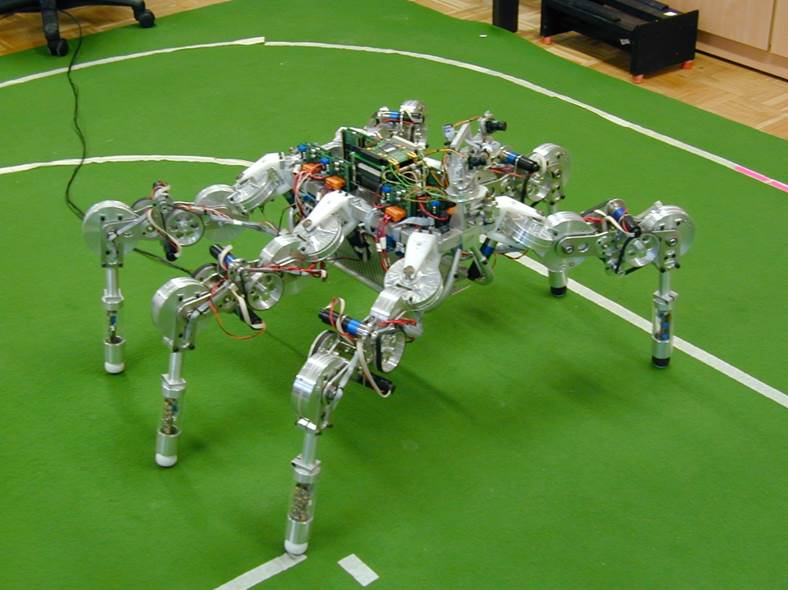
\includegraphics[width=6cm]{kapitel2/lauron3}
    \subcaption{Lauron III}\label{kap2:lauron3}
  \end{subfigure}%
  \qquad
  \begin{subfigure}[b]{.4\linewidth}
    \centering
    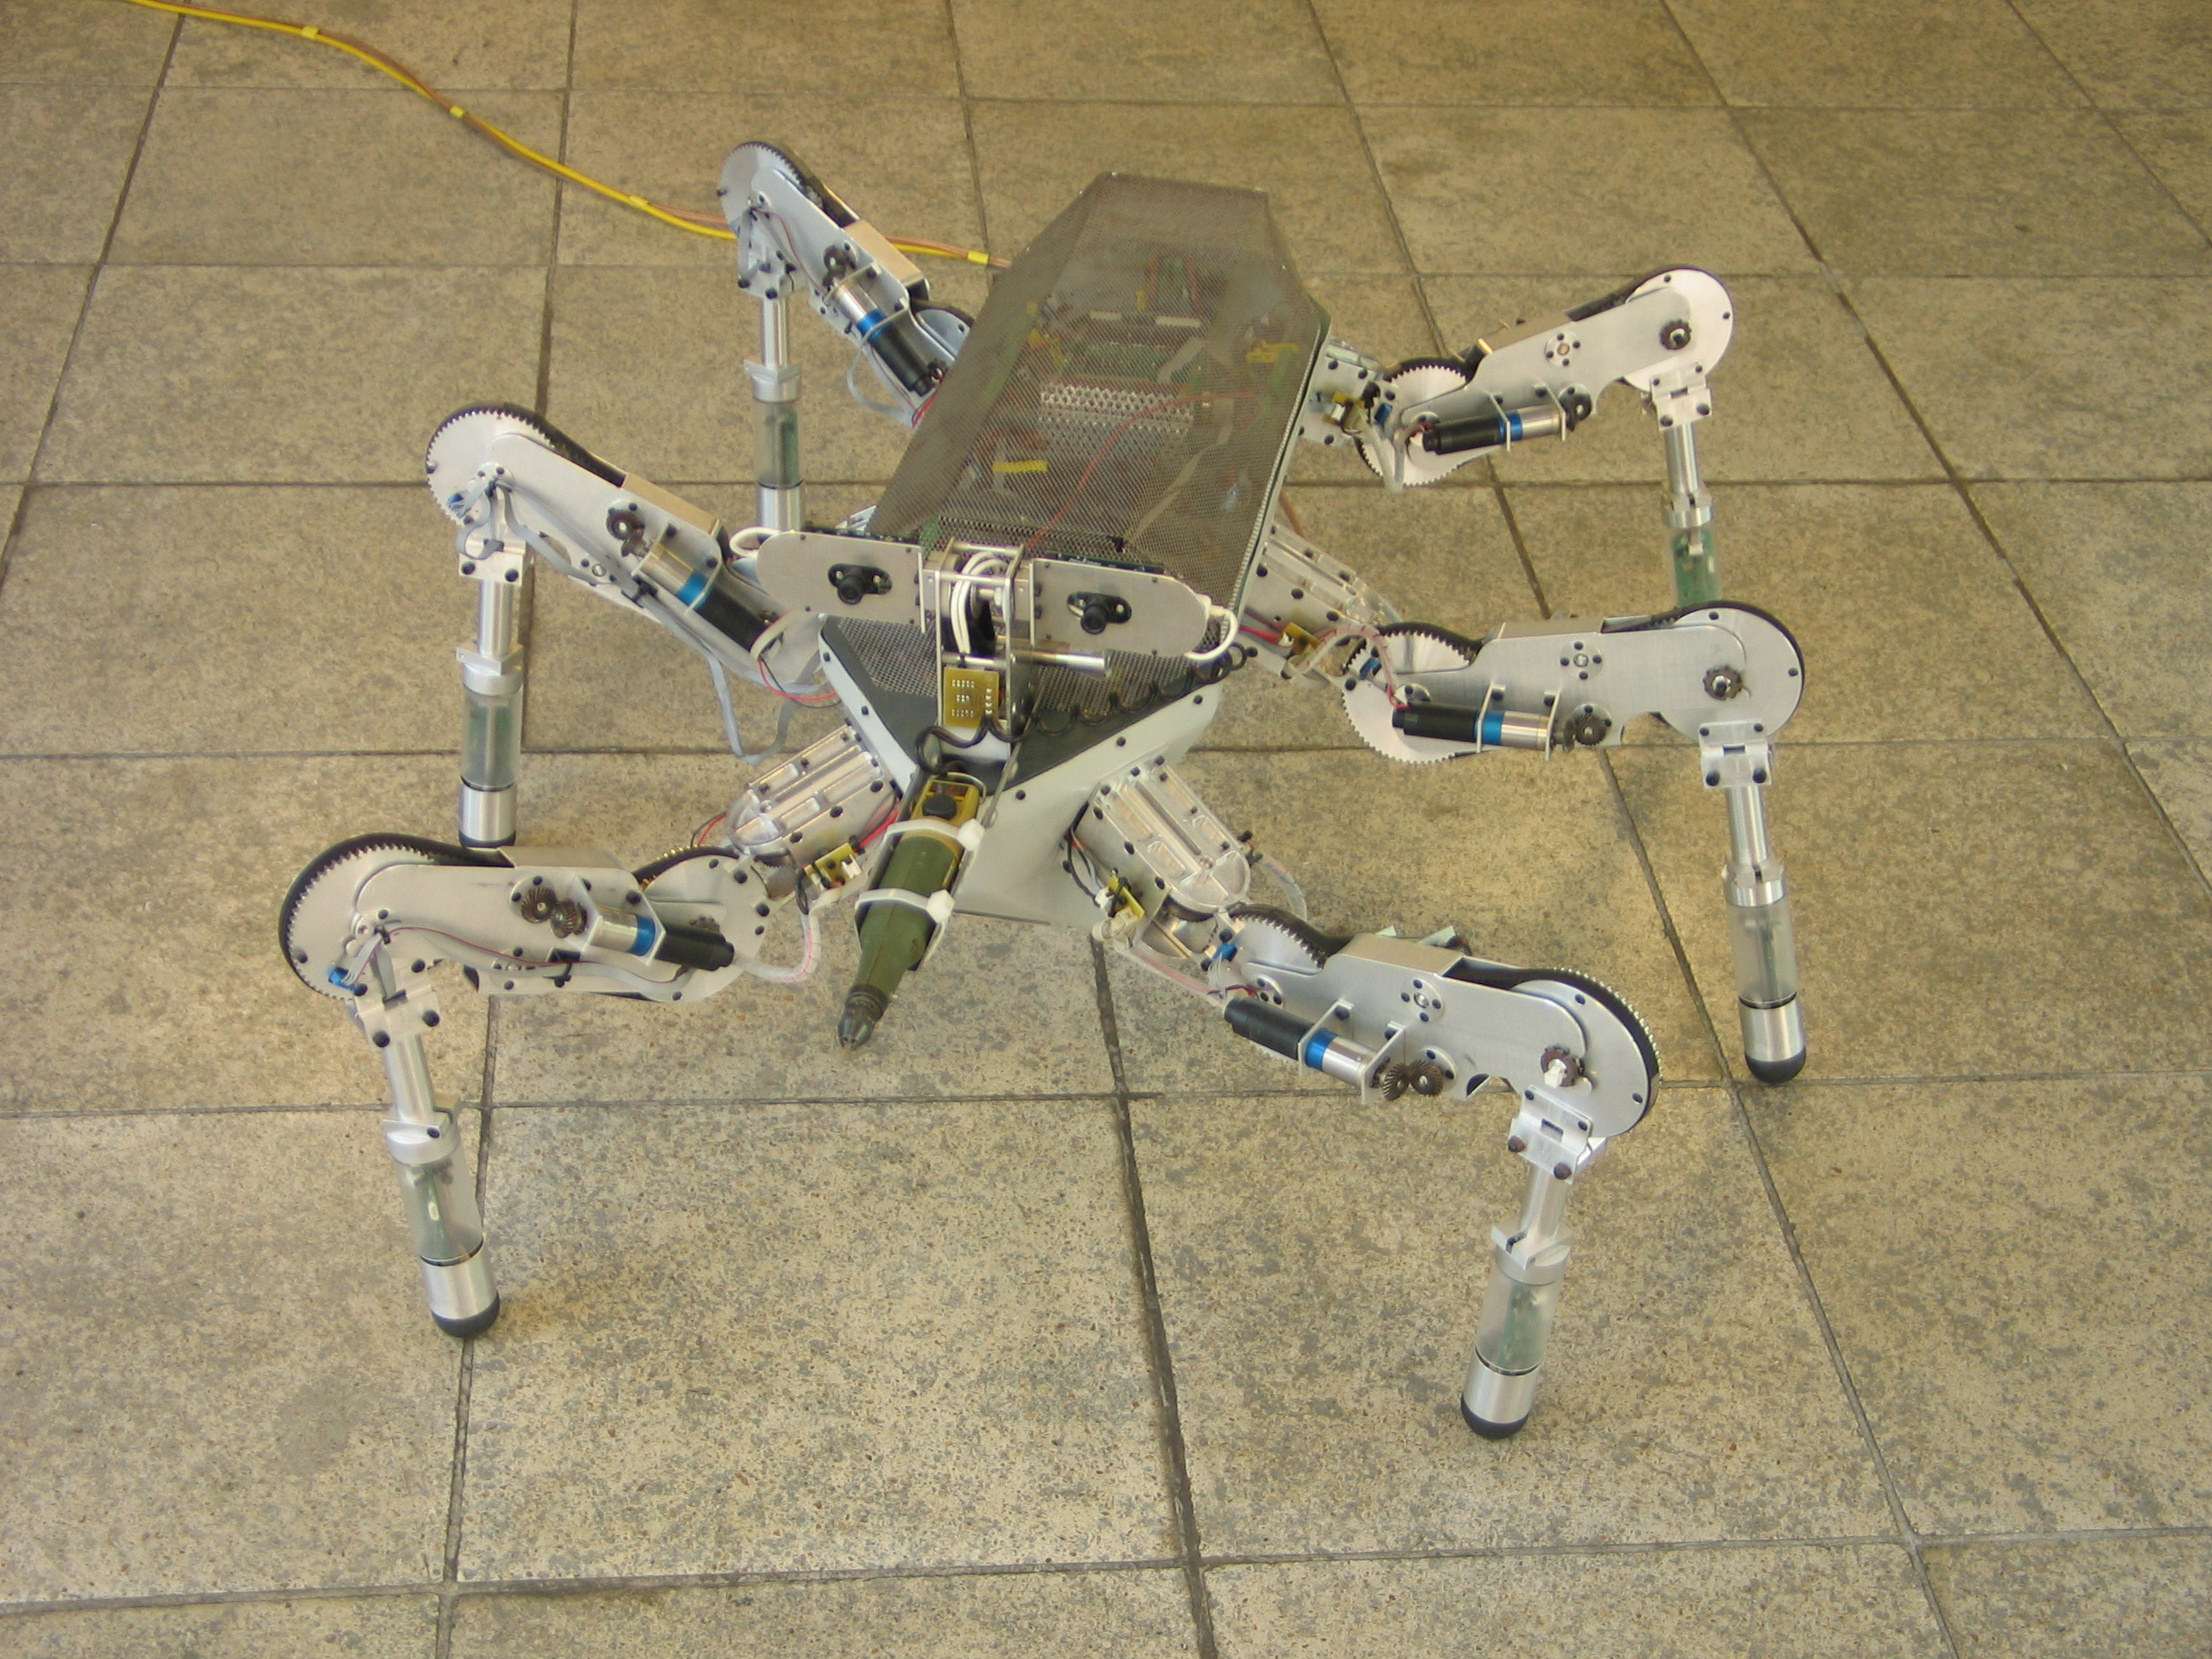
\includegraphics[width=6cm]{kapitel2/lauronivb}
    \subcaption{Lauron IVb}\label{kap2:lauron4b}
  \end{subfigure}\\
  \caption{Verschiedene Versionen des Lauron}
  \label{kap2lauron}
\end{figure}

Die Segmente sind durch die Gelenke Subcoxal $\alpha$, Coxa-Trochanter $\beta$ und Femur-Tibia $\gamma$ verbunden. Der Fuß jedes Beines wird Tarsus genannt. Das erste Gelenk Subcoxal besitzt zwei Freiheitsgrade, die weiteren Gelenke besitzen einen Freiheitsgrad. Damit ist für die indische Stabheuschrecke die minimale erforderliche Zahl an Freiheitsgraden erreicht, damit der Fuß beliebig im dreidimensionalen Raum gesetzt werden kann.

Unter anderem ist noch wichtig, dass der Kopf der indischen Stabheuschrecke zwei lange Fühler besitzt. Diese könnten in einem Roboter beispielsweise als Laserscanner oder Kamera modelliert werden, welche sich einen Überblick über die Gegend verschaffen können.

Der Körper des \emph{Lauron III} trägt die 7 Mikrocontroller (Infineon C167) und einen Hauptrechner, der auf Pentium basiert, die Akkumulatoren sowie den Kamerakopf. An beiden Seiten des Körpers sind jeweils drei Beine angebracht. Der Roboter wiegt 16 Kilogramm und hat eine maximale Zuladung von etwa 15kg. Die Maximalgeschwindigkeit beträgt \SI{0.5}{\metre\per\second}. \autocite{gassmann2000} \autocite{troilo2007}

\subsection{Akrobat}

\begin{figure}[b!]
  \centering
  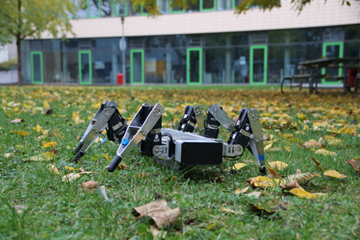
\includegraphics[height=8cm]{kapitel2/akrobat}
  \caption{Der Akrobat vor dem C-Gebäude der Hochschule Mannheim}
  \label{Kap2:akrobat}
\end{figure}

Auch der \emph{Akrobat} (\autoref{Kap2:akrobat}) ist der Form einer Stabheuschrecke nachempfunden und ähnelt in vielerlei Hinsicht dem Lauron.

Der Roboterkörper ist ungefähr 56 Millimeter hoch, 102 Millimeter breit und hat eine Seitenlänge von 62 Millimeter. Ebenfalls besitzt dieser sechs Beine mit je drei Segmenten. Diese haben die Längen 72 Millimeter, 97 Millimeter und 163 Millimeter, welche für kinematische Berechnungen von großer Bedeutung sind. Jedes Bein wiegt ungefähr 0,8 Kilogramm.

Jedes der Gelenke hat exakt einen Freiheitsgrad, sodass das gesamte Bein drei Freiheitsgrade hat. Wie auch beim Lauron ermöglicht dies die beliebige Positionierung im dreidimensionalen Raum. Die Gelenke sind mit dem Servomotor Dynamixel RX64 ausgestattet. Außerdem hat jedes Gelenk einen definierten Arbeitsbereich, welcher nicht unter- oder überschritten werden darf.
\begin{itemize}
  \item $\alpha$: -50$^\circ$ bis 50$^\circ$
  \item $\beta$: -106$^\circ$ bis 106$^\circ$
  \item $\gamma$: -135$^\circ$ bis 135$^\circ$
\end{itemize}  

Außerdem besitzt der Roboter am Kopf eine fest verbaute Kamera. Der Roboterkörper verfügt über genügend Freiraum für Batterien im mittleren Gehäuse. Im hinteren Gehäuse ist der Steuerrechner sowie die restliche Elektronik platziert.

Es handelt sich beim Rechner um den Einplatinencomputer Raspberry Pi (Modell B+) mit 512 MB Arbeitsspeicher und einem \SI{700}{MHz} ARM 11 Prozessor. Der Raspberry Pi bietet vielfältige Anschlussmöglichkeiten:
\begin{itemize}
\item Wireless Local Area Network (WLAN)
\item 4 Universal Serial Bus (USB)-Anschlüsse
\item 1 Ethernet-Anschluss
\item 1 High Definition Multimedia Interface (HDMI)-Anschluss, über den die Visualisierung mittels eines externen Bildschirms stattfindet
\item Camera Serial Interface (CSI)-Schnittstelle für die Kamera
\item Low Voltage Differential Signaling (LVDS)-Anschluss für die Ansteuerung von LCD-Displays
\item GPIO (General Purpose Input Output)-Anschlüsse
\end{itemize}

Es besteht die Möglichkeit, das Gamepad F710 von Logitech per WLAN anzuschließen. Theoretisch sind auch andere Gamepads möglich, sofern diese im Quellcode konfiguriert wurden. \autocite{askerow2014}

\section{Kinematik}

Um dem Roboter die richtigen Befehle zu senden, müssen als nächstes die Grundlagen für die Kinematik gesetzt werden. Ein Roboterbein entspricht jeweils einer kinematischen Kette, die aus mehreren starren Körpern besteht und die über Gelenke verbunden sind. Es handelt sich sowohl beim Lauron als auch beim Akrobat um Rotationsgelenke. Dieser Abschnitt beschreibt Methoden der Kinematik.

Mit Hilfe der direkten Kinematik lässt sich auf Grund der Gelenkausrichtungen berechnen, an welcher Position sich der sogenannte Endeffektor befindet. Der Endeffektor entspricht dem Fuß des Roboters. Über die inverse Kinematik kann bei einer gegebenen Fußposition berechnet werden, wie die Fußgelenke gestellt werden sollen. Die beschriebenen Methoden wurden bereits in weiterer Literatur erläutert. \autocite{den55} \autocite{wloka92} \autocite{ihme02} \autocite{fellmann2007}

\subsection{Denavit-Hartenberg-Verfahren}

Denavit und Hartenberg entwickelten ein Verfahren zur Beschreibung von kinematischen Ketten. Durch dieses Verfahren können mit Hilfe von nur vier Parametern, den DH-Parametern, die gegenseitige Lage zweier Elemente beschrieben werden. Dies macht die Berechnung von kinematischen Ketten wesentlich einfacher.

\begin{figure}[b!]
  \centering
  \begin{subfigure}[b]{.4\linewidth}
    \centering
    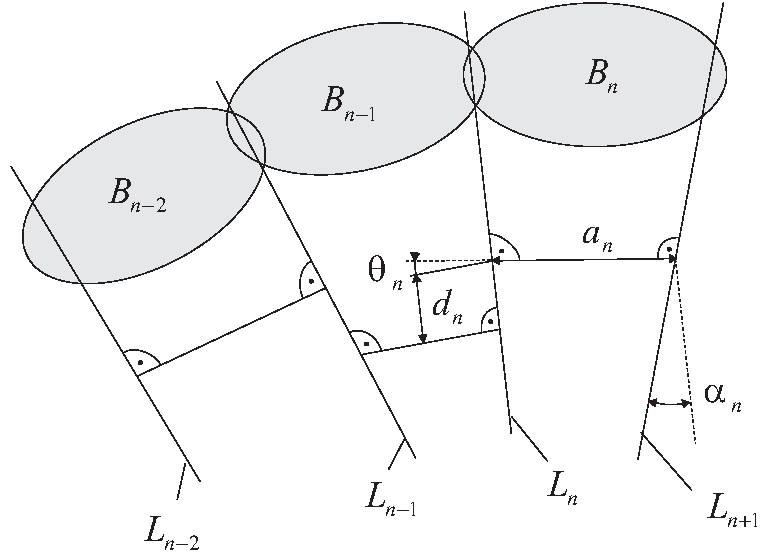
\includegraphics[width=6cm]{kapitel2/dh-parameter}
    \subcaption{Parameter}\label{kap2:dhparams}
  \end{subfigure}%
  \qquad
  \begin{subfigure}[b]{.4\linewidth}
    \centering
    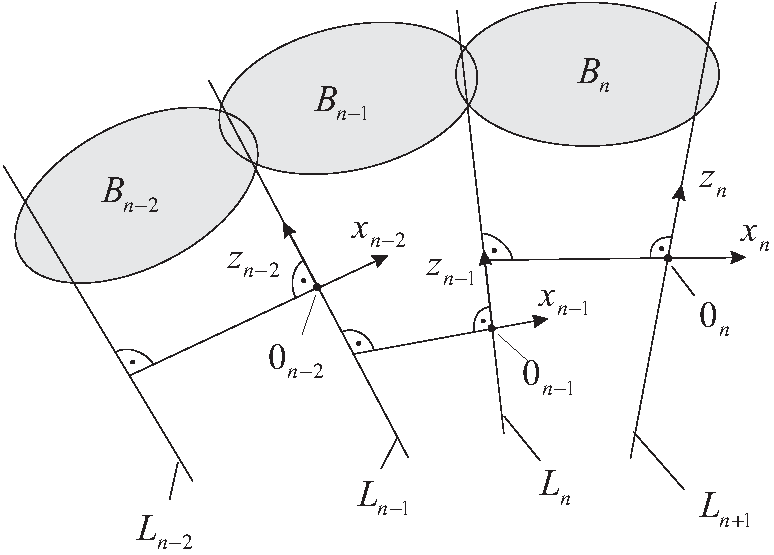
\includegraphics[width=6cm]{kapitel2/dh-koordinaten}
    \subcaption{Koordinatensysteme}\label{kap2:dhcoords}
  \end{subfigure}\\
  \caption{Denavit-Hartenberg Verfahren}
  \label{kap2lauron}
\end{figure}

Die vier Parameter (\autoref{kap2:dhparams}) können wie folgt berechnet werden:
\begin{enumerate}
  \item Entspricht der Länge der gemeinsamen Normale zwischen den Achsen $L_n$ und $L_{n+1}$. Dies ist im Schaubild die Variable $a_n$.
  \item Entspricht dem Versatz zwischen dieser und der vorherigen Normalen. Im Schaubild ist das die Variable $d_n$.
  \item Entspricht dem Drehwinkel zwischen $L_n$ und $L_{n+1}$. Im Schaubild ist das die Variable $\alpha_n$.
  \item Entspricht der Drehung um die Achse $L_n$. Im Schaubild ist dies die Variable $\theta_n$.
\end{enumerate} 

Des Weiteren ist es eine Voraussetzung für das Verfahren, dass für jedes Gelenk ein eigenes Koordinatensystem definiert ist (\autoref{kap2:dhcoords}), damit die Transformationsgleichungen aufgestellt werden können. Dabei ist es wichtig, dass eine Achse des Koordinatensystems auf der Gelenkachse und eine zweite auf der Normalen liegt. Damit sind nun alle Anforderungen erfüllt, um die direkte und die inverse Kinematik effizient zu berechnen.

\subsection{Direkte Kinematik}

\begin{figure}[b!]
  \centering
  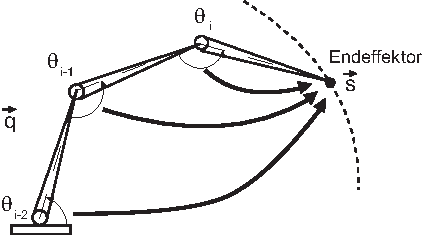
\includegraphics[height=5cm]{kapitel2/DirekteKinematik}
  \caption{Direkte Kinematik}
  \label{Kap2:direktekinematik}
\end{figure}

Mit Hilfe der direkten Kinematik lässt sich nun berechnen, an welcher Position sich der sogenannte Endeffektor befindet (\autoref{Kap2:direktekinematik}). Gegeben sind hierbei die Winkel der Gelenke. Der Vektor $ \vec{s} = (x,y,z,\alpha,\beta,\gamma)^T $  entspricht der Position und der Orientierung des Endeffektors. Der Vektor $ \vec{q} = (q_1, ...,q_n)^T $, bei dem $n$ die Anzahl der Gelenke ist, entspricht den Gelenkvariablen. Dann lässt sich die direkte Kinematik wie in \autoref{dk1} ausdrücken.
\begin{equation}
  \vec{s} = f(\vec{q})
\label{dk1}
\end{equation}

Mittels der DH-Parameter aus dem vorherigen Kapitel lässt sich nun eine homogene Transformationsmatrix vom Ausgangskoordinatensystem in das Koordinatensystem des Endeffektors abhängig der Gelenkvariablen, siehe \autoref{dk2}, erstellen.
\begin{equation}
  ^{n-1}_{n}T = \textrm{rot}(z_{n-1},\theta_n) \cdot \textrm{trans}(0,0,d_{n}) \cdot \textrm{trans}(a_{n},0,0) \cdot \textrm{rot}(x_{n},\alpha_{n})
\label{dk2}
\end{equation}

Der erste Parameter der Rotationsfunktion \textsc{rot} bestimmt die Rotationsachse. Der zweite Parameter bestimmt den Winkel. Die Funktion \textsc{trans} entspricht einer Verschiebung im Raum. Die Gleichung setzt voraus, dass die Wahl der Koordinatensysteme wie im vorherigen Kapitel beschrieben, eingehalten wird.

Als nächstes ersetzt man die Transformationen und Rotationen in \autoref{dk2} durch ihre homogenen Transformationenmatrizen und berechnet die gesamte Transformationsmatrix. Es ergibt sich das Ergebnis in \autoref{dk3} und \ref{dk3-2}, welche den Übergang vom Gelenk $n - 1$ in das Gelenk $n$ mit Hilfe der DH-Paramter beschreibt.
\begin{equation}
  ^{n-1}_{n}T = \begin{pmatrix}
    \textrm{cos}\: \theta_n & -\textrm{sin}\: \theta_n  & 0 & 0\\ 
    \textrm{sin}\: \theta_n & \textrm{cos}\: \theta_n   & 0 & 0\\ 
    0             & 0               & 1 & 0\\ 
    0             & 0               & 0 & 1\\
\end{pmatrix} \cdot
\begin{pmatrix}
  1 & 0 & 0 & a_n\\ 
  0 & 1 & 0 & 0\\ 
  0 & 0 & 1 & d_n\\ 
  0 & 0 & 0 & 1\\
\end{pmatrix} \cdot \begin{pmatrix}
  1 & 0 & 0 & 0\\ 
  0 & \textrm{cos}\: \alpha_n & -\textrm{sin}\: \alpha_n & 0\\ 
  0 & \textrm{sin}\: \alpha_n & \textrm{cos}\: \alpha_n & 0\\ 
  0 & 0 & 0 & 1\\
\end{pmatrix}
\label{dk3}
\end{equation}

\begin{equation}
^{n-1}_{n}T = \begin{pmatrix}
  \textrm{cos}\: \theta_n  & -\textrm{sin}\: \theta_n\; \textrm{cos}\: \alpha_n    & \textrm{sin}\: \theta_n\; \textrm{sin}\: \alpha_n & a_n\: \textrm{cos}\: \theta_n\\ 
  \textrm{sin}\: \theta_n  & \textrm{cos}\: \theta_n\; \textrm{cos}\: \alpha_n     & -\textrm{cos}\: \theta_n\; \textrm{sin}\: \alpha_n & a_n\: \textrm{sin}\: \theta_n\\ 
  0               & \textrm{sin}\: \alpha_n                & \textrm{cos}\: \alpha_n & d_n\\ 
  0               & 0                             & 0 & 1\\
\end{pmatrix}
\label{dk3-2}
\end{equation}

Da dies nur die Transformation zwischen einem und dem vorherigen Gelenk berechnet, muss nun die gesamte kinematische Kette in \autoref{dk4} hergestellt werden. Dies erfolgt durch die Multiplikation aller Einzeltransformationen.
\begin{equation}
  ^{0}_{m}T =\: ^{0}_{1}T \cdot \: ^{1}_{2}T \cdot \: ... ^{m-1}_{m}T
\label{dk4}
\end{equation}

Mit dieser Matrix kann ein Punkt im Koordinatensystem des Endeffektors in das Anfangskoordinatensystem transformiert werden. Ebenfalls lässt sich durch eine Aufteilung in Teilmatrizen die Orientierung und Position des Endeffektors relativ zum Anfangskoordinatensystem berechnen. Dazu dient \autoref{dk5}.
\begin{equation}
  _{m}^{0}T = \begin{pmatrix}
    _{m}^{0}R & ^{0}\vec{r}\\
    0 & 1\\
  \end{pmatrix}
\label{dk5}
\end{equation}

Dabei ist der Vektor $^{0}\vec{r}$ der gesuchte Vektor vom Koordinatensystem zum Endeffektor. Mit Hilfe der 3x3 Rotationsmatrix $_{m}^{0}R$, welche die Orientierung dieser Transformationen angibt, können die Winkel des Endeffektors berechnet werden. Dazu wird die Matrix noch aufgelöst. Durch das Auflösen des Gleichungssystems ergeben sich schlussendlich die folgenden Winkel in \autoref{dk6}:

\begin{equation}
  \begin{aligned}
    \alpha & = \textrm{arctan}(\alpha_{21} / \alpha_{11}) \\
    \beta & = \textrm{arctan}(-\alpha_{31} / (\alpha_{11} cos \gamma + \alpha_{21} sin \gamma)) \\
    \gamma & = \textrm{arctan}(\alpha_{32} / \alpha_{33})
  \end{aligned}
\label{dk6}
\end{equation}

\subsection{Inverse Kinematik}

\begin{figure}[b!]
  \centering
  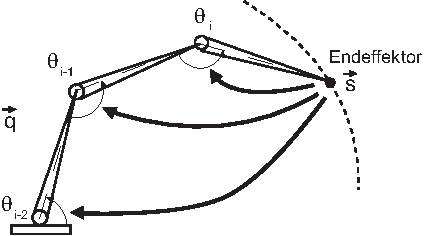
\includegraphics[height=5cm]{kapitel2/InverseKinematik}
  \caption{Inverse Kinematik}
  \label{Kap2:inversekinematik}
\end{figure}

Mit Hilfe der inversen Kinematik lässt sich nun berechnen, wie die Gelenkswinkel ausgerichtet werden müssen, damit der Endeffektor an eine bestimmte Position kommt (\autoref{Kap2:inversekinematik}). Dies ist gleichbedeutend mit der inversen Funktion der direkten Kinematik (\autoref{ik1}).
\begin{equation}
  \vec{q} = f^{-1}(\vec{s})
\label{ik1}
\end{equation}

Dabei ist zu beachten, dass es in den meisten Fällen für eine Eingabe mehrere Lösungen geben kann. Eine berechnete Lösung kann aber auch ungültig sein, wenn beispielsweise der Arbeitsbereich eingeschränkt ist oder Hindernisse auf dem Weg zur gewünschten Position liegen. Ebenfalls gibt es für viele Positionen auch gar keine Lösung. Des Weiteren kann die kinematische Kette durch Singularitäten Freiheitsgrade verlieren. Dies geschieht, wenn die Drehung an unterschiedlichen Achsen dieselbe Bewegung ergibt, dadurch, dass diese aufeinander liegen oder parallel verlaufen.

Da bereits die Funktion der direkten Kinematik eine nichtlineare Funktion ist, ist auch die inverse Funktion eine nichtlineare Funktion. Das Problem gehört damit in die Kategorie der Lösung eines nichtlinearen Gleichungssystems. Dies lässt sich über eine analytisches Verfahren oder annähernd über ein numerisches Verfahren lösen.

Bei der analytischen Methode wird versucht auf Basis der geometrischen Eigenschaften eine Formel herzuleiten. Dies wird umso schwerer, je mehr Freiheitsgrade die kinematische Kette hat. Der Vorteil liegt darin, dass die analytische Lösung ersten alle möglichen Gelenkstellungen für eine Position liefert und zweitens, dass sie wesentlich performanter ist. Die Lösungen sind exakt und Singularitäten können bereits beim Aufstellen der Gleichung festgestellt werden.

Die Software \emph{ikfast} \autocite{kanakia2012inverse} findet Lösungen und erstellt Gleichungen für die inverse Kinematik einer kinematischen Kette. Dabei nutzt die Software im Gegensatz zu anderer Software statt der numerischen die analytische Methode.

Bei der numerischen Lösung wird mittels einer linearen Annäherung versucht die Lösung für $f^{-1}$ zu finden. Dies lässt sich mit der Jacobi-Matrix berechnen. Dazu werden Teilfunktionen für $x$, $y$, $z$, $\alpha$, $\beta$ und $\gamma$ benötigt, welche sich aus der Transformationsmatrix der direkten Kinematik ergeben. Die Teilfunktionen werden dann nach jeder Variablen partiell abgeleitet. Dies ergibt die $6\:x\:n$ Jacobi-Matrix. Sie beschreibt die Änderung der Position des Endeffektors bei Änderung der Gelenkstellungen.

Durch weitere Umstellung der Funktion ergibt sich eine Gleichung für die lineare Annäherung an die gewünschte Funktion. Diese Lösung wird dann mittels direkter Kinematik überprüft. Ist die Abweichung zu groß, wird die Jacobi-Matrix mit den zuvor berechneten Gelenkstellungen erneut berechnet. Dies ergibt die lineare Annäherung an die Lösung. Wichtig ist dabei, dass eine maximale Zahl an Iterationen für den Algorithmus angegeben ist, da es manchmal auch gar keine Lösung geben kann.

Im Gegensatz zur analytischen Methode liefert die numerische Lösung immer nur einen Wert. Ein weiteres Problem der numerischen Lösung sind Singularitäten, welche auftreten können, wenn die Jacobi-Matrix an Rang verliert und somit singulär wird. Die Folge ist, dass die Matrix nicht mehr invertierbar ist und damit keine Lösung mehr berechnet werden kann. 

TODO: Formeln für analytische inverse Kinematik einbauen

\section{Laufplanung}

Nun werden die Grundlagen für die Laufplanung dargestellt. Dazu werden verschiedene reguläre Laufmuster und das freie Laufmuster Random Sampling dargestellt. Die regulären Laufmuster wurden in zahlreicher Literatur bei vielen Insekten beobachtet und auf das Thema Robotik übertragen. \autocite{ferrell1995comparison} \autocite{wilson1966insect} In der Robotik eignen sich diese, um auf ebenem Grund voranzuschreiten. Allerdings gibt es auch Untergründe, die stark uneben sind oder unüberwindbare Hindernisse aufweisen. Dann können freie Laufmuster wie Random Sampling zum Einsatz kommen.

\subsection{Reguläre Laufmuster}

Bei den regulären Laufmustern unterscheidet man zwischen drei häufig bei Insekten beobachteten Laufmustern, die aber alle der Gruppe \emph{wave gait} angehören:
\begin{itemize}
\item slow wave gait
\item ripple gait
\item tripod gait
\end{itemize}

Zunächst einmal müssen zwei Begriffe definiert werden, welche für die Betrachtung der Laufmuster wichtig sind. Diese entsprechen den beiden Phasen, welche die freien Laufmuster benötigen, um nach vorne zu laufen.
\begin{itemize}
\item \emph{power stroke}: In dieser Phase steht das Bein auf dem Boden und unterstützt die Körpermitte, sich nach vorne zu bewegen. Damit die Körpermitte sich nach vorne bewegen kann, wird das Bein in die entgegengesetzte Richtung gezogen, während es auf dem Boden bleibt.
\item \emph{return stroke}: Das Bein wird angehoben und nach vorne auf die nächste Position für die Ausführung der \emph{power stroke} gesetzt.
\end{itemize}

\begin{figure}[b!]
  \centering
  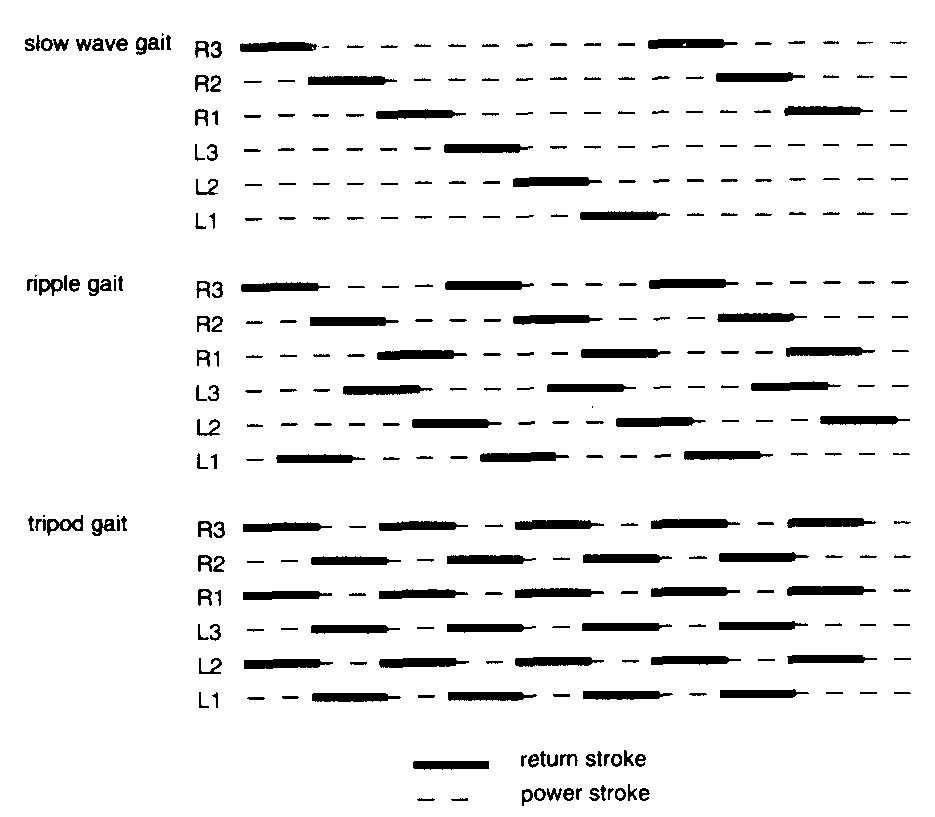
\includegraphics[height=8cm]{kapitel2/freie-gangarten}
  \caption{Reguläre Laufmuster von Insekten \autocite{ferrell1995comparison} \autocite{wilson1966insect}}
  \label{Kap2:laufmuster}
\end{figure}

\autoref{Kap2:laufmuster} zeigt nun für die drei Laufmuster zeitlich dargestellt, wann die \emph{power stroke} und wann die \emph{return stroke} ausgeführt wird.

Beim \emph{slow wave gait} befindet sich immer ein Bein in der \emph{return stroke}, während alle anderen sich in der \emph{power stroke} befinden und den Roboterkörper stützen und nach vorne bewegen. Auch die Reihenfolge spielt eine Rolle. Zuerst werden alle Beine einer Seite umgesetzt, dann erst alle der anderen Seite.

Beim \emph{ripple gait} werden um eine drittel Phase verschoben die Beine nacheinander umgesetzt. Daraus ergibt sich eine schnellere Bewegung als beim \emph{slow wave gait}. Auch hier spielt die Reihenfolge eine Rolle. Es wird immer abwechselnd ein Bein von links und dann ein Bein von rechts umgesetzt, während die anderen Beine in der \emph{power stroke} den Roboterkörper stützen und nach vorne bewegen.

Beim \emph{tripod gait} sind gleichzeitig drei Beine in der Phase \emph{power stroke}, während drei Beine in der Phase \emph{return stroke} sind. Bei der Auswahl müssen zwei Beine der einen Seite und ein Bein der anderen Seite ausgewählt werden, damit der Roboter nicht umfällt.

Da der \emph{tripod gait} die Phasen am schnellsten durchläuft, weil er immer die maximale Anzahl an möglichen Beinen gleichzeitig umsetzt oder stützen lässt, ist er in diesem Umfeld auch das schnellste der drei Laufmuster. Etwas langsamer ist der \emph{ripple gait}, während der \emph{slow wave gait} am langsamsten ist, da die Beine immer nur nacheinander umgesetzt werden.

\subsection{Freie Laufmuster}

Nun wird das freie Laufmuster \emph{Random Sampling} sowie einige weitere relevante Algorithmen vorgestellt. \autocite{herms2004}


\subsubsection{Random Sampling}

Beim Random Sampling werden zufällige gültige Lösungen generiert.  Wichtig ist, dass alle möglichen Lösungen generiert werden können und nur Lösungen ausgeschlossen werden, die außerhalb des gültigen Bereichs der Fußwinkel und Fußgeschwindigkeiten liegen, die auf instabilem Untergrund wie einem zu starkem Gefälle liegen oder die den Roboter zum Umkippen bringen würden.

Das Generieren von Lösungen erfolgt nun in mehreren Schritten. Zu Beginn müssen einige Berechnungen für die Festlegung des Pfades zum Ziel ablaufen, bevor der Hauptteil des Algorithmus abläuft, welcher sich schrittweise an das Ziel nähert, bis der Abstand zum Ziel annähernd null beträgt.

\paragraph{Festlegung des Pfades zum Ziel}

Eine erste Methode ist es, den Weg vom Start zum Ziel auf direktem Weg zu erreichen. Da allerdings nicht immer Lösungen auf direktem Weg möglich sind, müssen auch andere Pfade generiert werden. Beispielsweise könnte ein unüberwindbarer Graben oder eine hohe Mauer dafür sorgen, dass kein direkter Weg möglich ist. In diesem Fall müsste der Laufroboter den Weg um das Hindernis planen, um eine gültige Lösung zu finden. Um nun alle Fälle abzudecken, benötigt man eine zufällige Streckenplanung. Diese erfolgt, indem zuerst die Anzahl der Pfadsegmente festgelegt wird und dann genau so viele Wegpunkte gesetzt werden.

\paragraph{Festlegung der Anzahl der Pfadsegmente}

Die Festlegung der Anzahl der Pfadsegmente erfolgt über eine \emph{geometrische Verteilung}. Diese Verteilung wird genutzt, da geringe Streckenanzahlen häufig sein sollen, da davon ausgangen wird, dass der direkte Weg der schnellste Weg ist. Höhere Streckenanzahlen sollen weniger oft auftreten. Durch die Veränderung des Parameters $p$ lassen sich die Wahrscheinlichkeiten dahingehend variieren, dass entweder höhere oder niedrigere Streckenanzahlen bevorzugt werden. Standardmäßig geht man von p=\SI{0.5}{} aus, welches die Wahrscheinlichkeitsverteilung in \autoref{Kap3:streckenabschnittWahrscheinlichkeit} ergibt.

\begin{table}[t]
  \caption{Wahrscheinlichkeit der Anzahl der Pfadsegmente für die geplante Strecke}
  \label{Kap3:streckenabschnittWahrscheinlichkeit}
  \centering
  \sffamily
  \begin{footnotesize}
    \begin{tabular}{l S[table-format=1.3,table-comparator=true,table-space-text-post={***}]}
    \toprule
    \textbf{Anzahl Streckenabschnitte} & \textbf{Wahrscheinlichkeit in \%}\\
    \midrule
    1 & 50,0\\
    2 & 25,0\\
    3 & 12,5\\
    4 & 6,25\\
    5 & 3,125\\
    \bottomrule
    \end{tabular}
  \end{footnotesize}
  \rmfamily
\end{table}

\paragraph{Festlegung der Wegpunkte}

Nun ist definiert, wie viele Segmente der Pfad haben soll. Jetzt müssen die Wegpunkte auf dem Pfad zufällig generiert werden. Für jeden Pfadpunkt $P$ wird einzeln eine Lösung generiert. Zunächst wird der Mittelpunkt $m(x, y)$ sowie die Länge $l$ zwischen Start und Ende berechnet. Auf den Mittelpunkt wird nun ein zufälliger Vektor $r(x, y)$ addiert, dessen generierter Wert vom negativen bis zum positiven Betrag der Länge $l$ reicht. \autoref{RandomSamplingWegpunkteP1} und \ref{RandomSamplingWegpunkteP2} zeigen mögliche Ergebnisse für drei Pfadsegmente $P_1$, $P_2$ und $P_3$ für den Startpunkt $S(0,0)$ und dem Zielpunkt $Z(10,0)$. Der letzte Pfadpunkt $P_3$ entspricht immer genau der Zielposition, damit der Roboter dieses Ziel in jedem Fall erreicht. \autoref{Kap2:RSWegpunkte} zeigt die generierten Punkte und damit den Pfad des Roboters grafisch dargestellt.

\begin{equation}
  P_1=\left(\begin{array}{c} x_m + x_r \\ y_m + y_r \end{array}\right)=\left(\begin{array}{c} 5 - 2.31 \\ 0 - 4.1 \end{array}\right)=\left(\begin{array}{c} 3.31 \\ -4.1 \end{array}\right) \qquad
\label{RandomSamplingWegpunkteP1}
\end{equation}

\begin{equation}
  P_2=\left(\begin{array}{c} x_m + x_r \\ y_m + y_r \end{array}\right)=\left(\begin{array}{c} 5 + 3.1 \\ 0 + 0.5 \end{array}\right)=\left(\begin{array}{c} 8.1 \\ 0.5 \end{array}\right) \qquad
\label{RandomSamplingWegpunkteP2}
\end{equation}

\begin{figure}[t!]
  \centering
  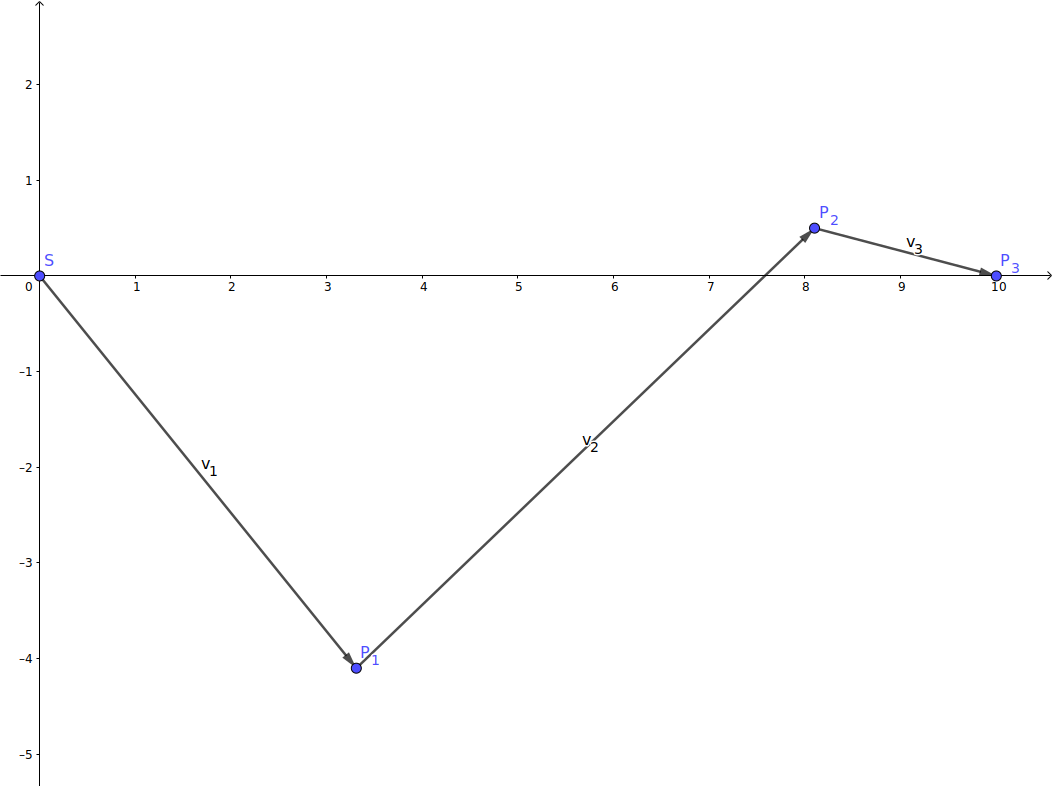
\includegraphics[width=1\textwidth]{kapitel2/rswegpunkte}
  \caption{Zufällig generierte Wegpunkte}
  \label{Kap2:RSWegpunkte}
\end{figure}

Mit dieser Berechnung sind nun für den Mittelpunkt des Körpers des Laufroboters ausschließlich Bewegungen auf diesem Pfad möglich. Bewusst wird hier noch nicht mit der z-Koordinate gearbeitet, da diese je nach Fußstellung und Terrain variiert.

\paragraph{Schrittweise Näherung an das Ziel}

Die schrittweise Näherung an das Ziel erfolgt solange, bis der Abstand zum Ziel minimal ist. Ein exakter Vergleich mit dem Abstand null ist nicht effektiv, da der Roboter sonst fortwährend versuchen würde auf seine Zielposition zu gelangen, aber ununterbrochen minimale Abweichungen zum Ziel hätte, was den Prozess erneut anstoßen würde. Der Ablauf, um die Füße anzuheben oder abzusetzen sowie den Körper zu bewegen, läuft folgendermaßen ab:
\begin{enumerate}
  \item Berechnung des zulässigen Bereichs
  \item Auswahl der nächsten Fuß-Konfiguration
\end{enumerate}

\paragraph{Berechnung des zulässigen Bereichs}

Der zulässige Bereich des Mittelpunkts ist auf Grund von zwei Kriterien eingeschränkt. Zum einen durch die maximalen Reichweite der Fußpunkte vom Mittelpunkt aus. Zum anderen dadurch, dass der minimale \emph{Stability Margin} nicht unterschritten werden darf. Der Stability Margin ist der kleinste Abstand zum Mittelpunkt der konvexen Hülle der Fußpunkte vom Mittelpunkt aus. Dieser ist ein Maß dafür, wie stabil der Roboter steht. Ist der Stability Margin kleiner als null, so ist der Mittelpunkt außerhalb der konvexen Hülle, was ein Kippen des Roboters verursacht. Je größer der Stability Margin, desto stabiler steht der Roboter.

Der zulässige Bereich kann nur an zwei Punkten verlassen werden. Damit wird ein Start- und ein Endpunkt der aktuellen Fußstellung gebildet. Diese sind analytisch schwer zu berechnen. Daher muss mit einem numerischen Verfahren, der \emph{binären Suche}, mit einem inneren zulässigen Punkt und einem äußerem unzulässigen Punkt der Schnittpunkt mit dem zulässigen Bereich gesucht werden. Dazu genügt eine Funktion welche angibt, ob der Mittelpunkt zulässig oder unzulässig ist.

\paragraph{Auswahl der nächsten Fuß-Konfiguration}

Der Mittelpunkt des Roboterkörpers kann sich in diesem aktuellen Zustand nur noch vom zuletzt berechneten Start- und Endpunkt des zulässigen Bereichs bewegen. Dies geschieht durch das Verschieben der Körpermitte. Dazu müssen die Füße gehoben und umgesetzt werden. Auch hier müssen die zu Beginn genannten Kriterien beachtet werden. Diese sind unter anderem, dass sich mindestens drei Füße auf dem Boden befinden und dass mindestens ein Fuß auf jeder Seite den Körper stützt, damit der Stability Margin positiv ist. Mit diesen Regeln lassen sich 40 mögliche Fußkonfigurationen, auch Stützzustände genannt, darstellen, welche in \autoref{validconf} abgebildet sind.

\begin{figure}[t!]
\setlength{\unitlength}{.9cm}
\begin{picture}(1.5,3.5)
\put(0.25,0.25){\dashbox{0.05}(1,2){} }
\put(0.25,1.25){\circle*{0.2}}
\put(1.25,1.25){\circle*{0.2}}
\put(1.25,0.25){\circle*{0.2}}
\put(1.25,0.25){\line(0,1){1}}
\put(0.25,1.25){\line(0,0){0}}
\put(0.25,1.25){\line(1, -1){1}}
\put(0.25,1.25){\line(1, 0){1}}
\put(0.75,2.5){\makebox(0,0)[b]{1}}
\end{picture}
\begin{picture}(1.5,3.5)
\put(0.25,0.25){\dashbox{0.05}(1,2){} }
\put(0.25,1.25){\circle*{0.2}}
\put(1.25,1.25){\circle*{0.2}}
\put(0.25,0.25){\circle*{0.2}}
\put(1.25,1.25){\line(0,0){0}}
\put(0.25,0.25){\line(0,1){1}}
\put(0.25,0.25){\line(1, 1){1}}
\put(0.25,1.25){\line(1, 0){1}}
\put(0.75,2.5){\makebox(0,0)[b]{2}}
\end{picture}
\begin{picture}(1.5,3.5)
\put(0.25,0.25){\dashbox{0.05}(1,2){} }
\put(0.25,2.25){\circle*{0.2}}
\put(0.25,1.25){\circle*{0.2}}
\put(1.25,1.25){\circle*{0.2}}
\put(1.25,1.25){\line(0,0){0}}
\put(0.25,1.25){\line(0,1){1}}
\put(0.25,1.25){\line(1, 0){1}}
\put(0.25,2.25){\line(1, -1){1}}
\put(0.75,2.5){\makebox(0,0)[b]{3}}
\end{picture}
\begin{picture}(1.5,3.5)
\put(0.25,0.25){\dashbox{0.05}(1,2){} }
\put(1.25,2.25){\circle*{0.2}}
\put(0.25,1.25){\circle*{0.2}}
\put(1.25,1.25){\circle*{0.2}}
\put(1.25,1.25){\line(0,1){1}}
\put(0.25,1.25){\line(0,0){0}}
\put(0.25,1.25){\line(1, 0){1}}
\put(0.25,1.25){\line(1, 1){1}}
\put(0.75,2.5){\makebox(0,0)[b]{4}}
\end{picture}
\begin{picture}(1.5,3.5)
\put(0.25,0.25){\dashbox{0.05}(1,2){} }
\put(1.25,1.25){\circle*{0.2}}
\put(0.25,0.25){\circle*{0.2}}
\put(1.25,0.25){\circle*{0.2}}
\put(1.25,0.25){\line(0,1){1}}
\put(0.25,0.25){\line(0,0){0}}
\put(0.25,0.25){\line(1, 0){1}}
\put(0.25,0.25){\line(1, 1){1}}
\put(0.75,2.5){\makebox(0,0)[b]{5}}
\end{picture}
\begin{picture}(1.5,3.5)
\put(0.25,0.25){\dashbox{0.05}(1,2){} }
\put(0.25,1.25){\circle*{0.2}}
\put(0.25,0.25){\circle*{0.2}}
\put(1.25,0.25){\circle*{0.2}}
\put(1.25,0.25){\line(0,0){0}}
\put(0.25,0.25){\line(0,1){1}}
\put(0.25,0.25){\line(1, 0){1}}
\put(0.25,1.25){\line(1, -1){1}}
\put(0.75,2.5){\makebox(0,0)[b]{6}}
\end{picture}
\begin{picture}(1.5,3.5)
\put(0.25,0.25){\dashbox{0.05}(1,2){} }
\put(0.25,2.25){\circle*{0.2}}
\put(1.25,2.25){\circle*{0.2}}
\put(1.25,1.25){\circle*{0.2}}
\put(1.25,1.25){\line(0,1){1}}
\put(0.25,2.25){\line(0,0){0}}
\put(0.25,2.25){\line(1, -1){1}}
\put(0.25,2.25){\line(1, 0){1}}
\put(0.75,2.5){\makebox(0,0)[b]{7}}
\end{picture}
\begin{picture}(1.5,3.5)
\put(0.25,0.25){\dashbox{0.05}(1,2){} }
\put(0.25,2.25){\circle*{0.2}}
\put(1.25,2.25){\circle*{0.2}}
\put(0.25,1.25){\circle*{0.2}}
\put(1.25,2.25){\line(0,0){0}}
\put(0.25,1.25){\line(0,1){1}}
\put(0.25,1.25){\line(1, 1){1}}
\put(0.25,2.25){\line(1, 0){1}}
\put(0.75,2.5){\makebox(0,0)[b]{8}}
\end{picture}
\begin{picture}(1.5,3.5)
\put(0.25,0.25){\dashbox{0.05}(1,2){} }
\put(1.25,2.25){\circle*{0.2}}
\put(1.25,1.25){\circle*{0.2}}
\put(0.25,0.25){\circle*{0.2}}
\put(1.25,1.25){\line(0,1){1}}
\put(0.25,0.25){\line(0,0){0}}
\put(0.25,0.25){\line(1, 1){1}}
\put(0.25,0.25){\line(1, 2){1}}
\put(0.75,2.5){\makebox(0,0)[b]{9}}
\end{picture}
\begin{picture}(1.5,3.5)
\put(0.25,0.25){\dashbox{0.05}(1,2){} }
\put(1.25,2.25){\circle*{0.2}}
\put(0.25,1.25){\circle*{0.2}}
\put(0.25,0.25){\circle*{0.2}}
\put(1.25,2.25){\line(0,0){0}}
\put(0.25,0.25){\line(0,1){1}}
\put(0.25,0.25){\line(1, 2){1}}
\put(0.25,1.25){\line(1, 1){1}}
\put(0.75,2.5){\makebox(0,0)[b]{10}}
\end{picture}
\begin{picture}(1.5,3.5)
\put(0.25,0.25){\dashbox{0.05}(1,2){} }
\put(0.25,2.25){\circle*{0.2}}
\put(1.25,1.25){\circle*{0.2}}
\put(1.25,0.25){\circle*{0.2}}
\put(1.25,0.25){\line(0,1){1}}
\put(0.25,2.25){\line(0,0){0}}
\put(0.25,2.25){\line(1, -2){1}}
\put(0.25,2.25){\line(1, -1){1}}
\put(0.75,2.5){\makebox(0,0)[b]{11}}
\end{picture}
\begin{picture}(1.5,3.5)
\put(0.25,0.25){\dashbox{0.05}(1,2){} }
\put(0.25,2.25){\circle*{0.2}}
\put(0.25,1.25){\circle*{0.2}}
\put(1.25,0.25){\circle*{0.2}}
\put(1.25,0.25){\line(0,0){0}}
\put(0.25,1.25){\line(0,1){1}}
\put(0.25,1.25){\line(1, -1){1}}
\put(0.25,2.25){\line(1, -2){1}}
\put(0.75,2.5){\makebox(0,0)[b]{12}}
\end{picture}
\begin{picture}(1.5,3.5)
\put(0.25,0.25){\dashbox{0.05}(1,2){} }
\put(0.25,2.25){\circle*{0.2}}
\put(1.25,2.25){\circle*{0.2}}
\put(1.25,0.25){\circle*{0.2}}
\put(1.25,0.25){\line(0,2){2}}
\put(0.25,2.25){\line(0,0){0}}
\put(0.25,2.25){\line(1, -2){1}}
\put(0.25,2.25){\line(1, 0){1}}
\put(0.75,2.5){\makebox(0,0)[b]{13}}
\end{picture}
\begin{picture}(1.5,3.5)
\put(0.25,0.25){\dashbox{0.05}(1,2){} }
\put(1.25,2.25){\circle*{0.2}}
\put(0.25,0.25){\circle*{0.2}}
\put(1.25,0.25){\circle*{0.2}}
\put(1.25,0.25){\line(0,2){2}}
\put(0.25,0.25){\line(0,0){0}}
\put(0.25,0.25){\line(1, 0){1}}
\put(0.25,0.25){\line(1, 2){1}}
\put(0.75,2.5){\makebox(0,0)[b]{14}}
\end{picture}
\begin{picture}(1.5,3.5)
\put(0.25,0.25){\dashbox{0.05}(1,2){} }
\put(0.25,2.25){\circle*{0.2}}
\put(1.25,2.25){\circle*{0.2}}
\put(0.25,0.25){\circle*{0.2}}
\put(1.25,2.25){\line(0,0){0}}
\put(0.25,0.25){\line(0,2){2}}
\put(0.25,0.25){\line(1, 2){1}}
\put(0.25,2.25){\line(1, 0){1}}
\put(0.75,2.5){\makebox(0,0)[b]{15}}
\end{picture}
\begin{picture}(1.5,3.5)
\put(0.25,0.25){\dashbox{0.05}(1,2){} }
\put(0.25,2.25){\circle*{0.2}}
\put(0.25,0.25){\circle*{0.2}}
\put(1.25,0.25){\circle*{0.2}}
\put(1.25,0.25){\line(0,0){0}}
\put(0.25,0.25){\line(0,2){2}}
\put(0.25,0.25){\line(1, 0){1}}
\put(0.25,2.25){\line(1, -2){1}}
\put(0.75,2.5){\makebox(0,0)[b]{16}}
\end{picture}
\begin{picture}(1.5,3.5)
\put(0.25,0.25){\dashbox{0.05}(1,2){} }
\put(1.25,2.25){\circle*{0.2}}
\put(0.25,1.25){\circle*{0.2}}
\put(1.25,0.25){\circle*{0.2}}
\put(1.25,0.25){\line(0,2){2}}
\put(0.25,1.25){\line(0,0){0}}
\put(0.25,1.25){\line(1, -1){1}}
\put(0.25,1.25){\line(1, 1){1}}
\put(0.75,2.5){\makebox(0,0)[b]{17}}
\end{picture}
\begin{picture}(1.5,3.5)
\put(0.25,0.25){\dashbox{0.05}(1,2){} }
\put(0.25,2.25){\circle*{0.2}}
\put(1.25,1.25){\circle*{0.2}}
\put(0.25,0.25){\circle*{0.2}}
\put(1.25,1.25){\line(0,0){0}}
\put(0.25,0.25){\line(0,2){2}}
\put(0.25,0.25){\line(1, 1){1}}
\put(0.25,2.25){\line(1, -1){1}}
\put(0.75,2.5){\makebox(0,0)[b]{18}}
\end{picture}
\begin{picture}(1.5,3.5)
\put(0.25,0.25){\dashbox{0.05}(1,2){} }
\put(0.25,2.25){\circle*{0.2}}
\put(0.25,1.25){\circle*{0.2}}
\put(1.25,1.25){\circle*{0.2}}
\put(0.25,0.25){\circle*{0.2}}
\put(1.25,1.25){\line(0,0){0}}
\put(0.25,0.25){\line(0,2){2}}
\put(0.25,0.25){\line(1, 1){1}}
\put(0.25,2.25){\line(1, -1){1}}
\put(0.75,2.5){\makebox(0,0)[b]{19}}
\end{picture}
\begin{picture}(1.5,3.5)
\put(0.25,0.25){\dashbox{0.05}(1,2){} }
\put(1.25,2.25){\circle*{0.2}}
\put(0.25,1.25){\circle*{0.2}}
\put(1.25,1.25){\circle*{0.2}}
\put(1.25,0.25){\circle*{0.2}}
\put(1.25,0.25){\line(0,2){2}}
\put(0.25,1.25){\line(0,0){0}}
\put(0.25,1.25){\line(1, -1){1}}
\put(0.25,1.25){\line(1, 1){1}}
\put(0.75,2.5){\makebox(0,0)[b]{20}}
\end{picture}
\begin{picture}(1.5,3.5)
\put(0.25,0.25){\dashbox{0.05}(1,2){} }
\put(1.25,2.25){\circle*{0.2}}
\put(1.25,1.25){\circle*{0.2}}
\put(0.25,0.25){\circle*{0.2}}
\put(1.25,0.25){\circle*{0.2}}
\put(1.25,0.25){\line(0,2){2}}
\put(0.25,0.25){\line(0,0){0}}
\put(0.25,0.25){\line(1, 0){1}}
\put(0.25,0.25){\line(1, 2){1}}
\put(0.75,2.5){\makebox(0,0)[b]{21}}
\end{picture}
\begin{picture}(1.5,3.5)
\put(0.25,0.25){\dashbox{0.05}(1,2){} }
\put(0.25,2.25){\circle*{0.2}}
\put(0.25,1.25){\circle*{0.2}}
\put(0.25,0.25){\circle*{0.2}}
\put(1.25,0.25){\circle*{0.2}}
\put(1.25,0.25){\line(0,0){0}}
\put(0.25,0.25){\line(0,2){2}}
\put(0.25,0.25){\line(1, 0){1}}
\put(0.25,2.25){\line(1, -2){1}}
\put(0.75,2.5){\makebox(0,0)[b]{22}}
\end{picture}
\begin{picture}(1.5,3.5)
\put(0.25,0.25){\dashbox{0.05}(1,2){} }
\put(0.25,2.25){\circle*{0.2}}
\put(1.25,2.25){\circle*{0.2}}
\put(1.25,1.25){\circle*{0.2}}
\put(1.25,0.25){\circle*{0.2}}
\put(1.25,0.25){\line(0,2){2}}
\put(0.25,2.25){\line(0,0){0}}
\put(0.25,2.25){\line(1, -2){1}}
\put(0.25,2.25){\line(1, 0){1}}
\put(0.75,2.5){\makebox(0,0)[b]{23}}
\end{picture}
\begin{picture}(1.5,3.5)
\put(0.25,0.25){\dashbox{0.05}(1,2){} }
\put(0.25,2.25){\circle*{0.2}}
\put(1.25,2.25){\circle*{0.2}}
\put(0.25,1.25){\circle*{0.2}}
\put(0.25,0.25){\circle*{0.2}}
\put(1.25,2.25){\line(0,0){0}}
\put(0.25,0.25){\line(0,2){2}}
\put(0.25,0.25){\line(1, 2){1}}
\put(0.25,2.25){\line(1, 0){1}}
\put(0.75,2.5){\makebox(0,0)[b]{24}}
\end{picture}
\begin{picture}(1.5,3.5)
\put(0.25,0.25){\dashbox{0.05}(1,2){} }
\put(0.25,2.25){\circle*{0.2}}
\put(1.25,2.25){\circle*{0.2}}
\put(0.25,1.25){\circle*{0.2}}
\put(1.25,1.25){\circle*{0.2}}
\put(1.25,1.25){\line(0,1){1}}
\put(0.25,1.25){\line(0,1){1}}
\put(0.25,1.25){\line(1, 0){1}}
\put(0.25,2.25){\line(1, 0){1}}
\put(0.75,2.5){\makebox(0,0)[b]{25}}
\end{picture}
\begin{picture}(1.5,3.5)
\put(0.25,0.25){\dashbox{0.05}(1,2){} }
\put(0.25,1.25){\circle*{0.2}}
\put(1.25,1.25){\circle*{0.2}}
\put(0.25,0.25){\circle*{0.2}}
\put(1.25,0.25){\circle*{0.2}}
\put(1.25,0.25){\line(0,1){1}}
\put(0.25,0.25){\line(0,1){1}}
\put(0.25,0.25){\line(1, 0){1}}
\put(0.25,1.25){\line(1, 0){1}}
\put(0.75,2.5){\makebox(0,0)[b]{26}}
\end{picture}
\begin{picture}(1.5,3.5)
\put(0.25,0.25){\dashbox{0.05}(1,2){} }
\put(1.25,2.25){\circle*{0.2}}
\put(0.25,1.25){\circle*{0.2}}
\put(1.25,1.25){\circle*{0.2}}
\put(0.25,0.25){\circle*{0.2}}
\put(1.25,1.25){\line(0,1){1}}
\put(0.25,0.25){\line(0,1){1}}
\put(0.25,0.25){\line(1, 1){1}}
\put(0.25,1.25){\line(1, 1){1}}
\put(0.75,2.5){\makebox(0,0)[b]{27}}
\end{picture}
\begin{picture}(1.5,3.5)
\put(0.25,0.25){\dashbox{0.05}(1,2){} }
\put(0.25,2.25){\circle*{0.2}}
\put(0.25,1.25){\circle*{0.2}}
\put(1.25,1.25){\circle*{0.2}}
\put(1.25,0.25){\circle*{0.2}}
\put(1.25,0.25){\line(0,1){1}}
\put(0.25,1.25){\line(0,1){1}}
\put(0.25,1.25){\line(1, -1){1}}
\put(0.25,2.25){\line(1, -1){1}}
\put(0.75,2.5){\makebox(0,0)[b]{28}}
\end{picture}
\begin{picture}(1.5,3.5)
\put(0.25,0.25){\dashbox{0.05}(1,2){} }
\put(1.25,2.25){\circle*{0.2}}
\put(0.25,1.25){\circle*{0.2}}
\put(0.25,0.25){\circle*{0.2}}
\put(1.25,0.25){\circle*{0.2}}
\put(1.25,0.25){\line(0,2){2}}
\put(0.25,0.25){\line(0,1){1}}
\put(0.25,0.25){\line(1, 0){1}}
\put(0.25,1.25){\line(1, 1){1}}
\put(0.75,2.5){\makebox(0,0)[b]{29}}
\end{picture}
\begin{picture}(1.5,3.5)
\put(0.25,0.25){\dashbox{0.05}(1,2){} }
\put(0.25,2.25){\circle*{0.2}}
\put(1.25,1.25){\circle*{0.2}}
\put(0.25,0.25){\circle*{0.2}}
\put(1.25,0.25){\circle*{0.2}}
\put(1.25,0.25){\line(0,1){1}}
\put(0.25,0.25){\line(0,2){2}}
\put(0.25,0.25){\line(1, 0){1}}
\put(0.25,2.25){\line(1, -1){1}}
\put(0.75,2.5){\makebox(0,0)[b]{30}}
\end{picture}
\begin{picture}(1.5,3.5)
\put(0.25,0.25){\dashbox{0.05}(1,2){} }
\put(0.25,2.25){\circle*{0.2}}
\put(1.25,2.25){\circle*{0.2}}
\put(0.25,1.25){\circle*{0.2}}
\put(1.25,0.25){\circle*{0.2}}
\put(1.25,0.25){\line(0,2){2}}
\put(0.25,1.25){\line(0,1){1}}
\put(0.25,1.25){\line(1, -1){1}}
\put(0.25,2.25){\line(1, 0){1}}
\put(0.75,2.5){\makebox(0,0)[b]{31}}
\end{picture}
\begin{picture}(1.5,3.5)
\put(0.25,0.25){\dashbox{0.05}(1,2){} }
\put(0.25,2.25){\circle*{0.2}}
\put(1.25,2.25){\circle*{0.2}}
\put(1.25,1.25){\circle*{0.2}}
\put(0.25,0.25){\circle*{0.2}}
\put(1.25,1.25){\line(0,1){1}}
\put(0.25,0.25){\line(0,2){2}}
\put(0.25,0.25){\line(1, 1){1}}
\put(0.25,2.25){\line(1, 0){1}}
\put(0.75,2.5){\makebox(0,0)[b]{32}}
\end{picture}
\begin{picture}(1.5,3.5)
\put(0.25,0.25){\dashbox{0.05}(1,2){} }
\put(0.25,2.25){\circle*{0.2}}
\put(1.25,2.25){\circle*{0.2}}
\put(0.25,0.25){\circle*{0.2}}
\put(1.25,0.25){\circle*{0.2}}
\put(1.25,0.25){\line(0,2){2}}
\put(0.25,0.25){\line(0,2){2}}
\put(0.25,0.25){\line(1, 0){1}}
\put(0.25,2.25){\line(1, 0){1}}
\put(0.75,2.5){\makebox(0,0)[b]{33}}
\end{picture}
\begin{picture}(1.5,3.5)
\put(0.25,0.25){\dashbox{0.05}(1,2){} }
\put(1.25,2.25){\circle*{0.2}}
\put(0.25,1.25){\circle*{0.2}}
\put(1.25,1.25){\circle*{0.2}}
\put(0.25,0.25){\circle*{0.2}}
\put(1.25,0.25){\circle*{0.2}}
\put(1.25,0.25){\line(0,2){2}}
\put(0.25,0.25){\line(0,1){1}}
\put(0.25,0.25){\line(1, 0){1}}
\put(0.25,1.25){\line(1, 1){1}}
\put(0.75,2.5){\makebox(0,0)[b]{34}}
\end{picture}
\begin{picture}(1.5,3.5)
\put(0.25,0.25){\dashbox{0.05}(1,2){} }
\put(0.25,2.25){\circle*{0.2}}
\put(0.25,1.25){\circle*{0.2}}
\put(1.25,1.25){\circle*{0.2}}
\put(0.25,0.25){\circle*{0.2}}
\put(1.25,0.25){\circle*{0.2}}
\put(1.25,0.25){\line(0,1){1}}
\put(0.25,0.25){\line(0,2){2}}
\put(0.25,0.25){\line(1, 0){1}}
\put(0.25,2.25){\line(1, -1){1}}
\put(0.75,2.5){\makebox(0,0)[b]{35}}
\end{picture}
\begin{picture}(1.5,3.5)
\put(0.25,0.25){\dashbox{0.05}(1,2){} }
\put(0.25,2.25){\circle*{0.2}}
\put(1.25,2.25){\circle*{0.2}}
\put(0.25,1.25){\circle*{0.2}}
\put(1.25,1.25){\circle*{0.2}}
\put(1.25,0.25){\circle*{0.2}}
\put(1.25,0.25){\line(0,2){2}}
\put(0.25,1.25){\line(0,1){1}}
\put(0.25,1.25){\line(1, -1){1}}
\put(0.25,2.25){\line(1, 0){1}}
\put(0.75,2.5){\makebox(0,0)[b]{36}}
\end{picture}
\begin{picture}(1.5,3.5)
\put(0.25,0.25){\dashbox{0.05}(1,2){} }
\put(0.25,2.25){\circle*{0.2}}
\put(1.25,2.25){\circle*{0.2}}
\put(0.25,1.25){\circle*{0.2}}
\put(1.25,1.25){\circle*{0.2}}
\put(0.25,0.25){\circle*{0.2}}
\put(1.25,1.25){\line(0,1){1}}
\put(0.25,0.25){\line(0,2){2}}
\put(0.25,0.25){\line(1, 1){1}}
\put(0.25,2.25){\line(1, 0){1}}
\put(0.75,2.5){\makebox(0,0)[b]{37}}
\end{picture}
\begin{picture}(1.5,3.5)
\put(0.25,0.25){\dashbox{0.05}(1,2){} }
\put(0.25,2.25){\circle*{0.2}}
\put(1.25,2.25){\circle*{0.2}}
\put(1.25,1.25){\circle*{0.2}}
\put(0.25,0.25){\circle*{0.2}}
\put(1.25,0.25){\circle*{0.2}}
\put(1.25,0.25){\line(0,2){2}}
\put(0.25,0.25){\line(0,2){2}}
\put(0.25,0.25){\line(1, 0){1}}
\put(0.25,2.25){\line(1, 0){1}}
\put(0.75,2.5){\makebox(0,0)[b]{38}}
\end{picture}
\begin{picture}(1.5,3.5)
\put(0.25,0.25){\dashbox{0.05}(1,2){} }
\put(0.25,2.25){\circle*{0.2}}
\put(1.25,2.25){\circle*{0.2}}
\put(0.25,1.25){\circle*{0.2}}
\put(0.25,0.25){\circle*{0.2}}
\put(1.25,0.25){\circle*{0.2}}
\put(1.25,0.25){\line(0,2){2}}
\put(0.25,0.25){\line(0,2){2}}
\put(0.25,0.25){\line(1, 0){1}}
\put(0.25,2.25){\line(1, 0){1}}
\put(0.75,2.5){\makebox(0,0)[b]{39}}
\end{picture}
\begin{picture}(1.5,3.5)
\put(0.25,0.25){\dashbox{0.05}(1,2){} }
\put(0.25,2.25){\circle*{0.2}}
\put(1.25,2.25){\circle*{0.2}}
\put(0.25,1.25){\circle*{0.2}}
\put(1.25,1.25){\circle*{0.2}}
\put(0.25,0.25){\circle*{0.2}}
\put(1.25,0.25){\circle*{0.2}}
\put(1.25,0.25){\line(0,2){2}}
\put(0.25,0.25){\line(0,2){2}}
\put(0.25,0.25){\line(1, 0){1}}
\put(0.25,2.25){\line(1, 0){1}}
\put(0.75,2.5){\makebox(0,0)[b]{40}}
\end{picture}
\caption{\label{validconf}40 zulässige Stützzustände \autocite{herms2004}}
\end{figure}

Mit jedem Übergang eines Stützzustands in einen anderen Stützzustands wird exakt ein Fuß entweder angehoben oder abgesetzt. Es können auch mehrere Füße gleichzeitig angehoben oder abgesetzt werden, indem in dem aktuellen Übergang eine Zeitdauer von \SI{0}{s} angenommen wird. Damit wird der nächste Stützzustand mit dem aktuellen Stützzustand ausgeführt. \autoref{trans_support} gibt alle möglichen Stützzustände an.

\begin{table}[t!]
  \caption{\label{trans_support} Transitionstabelle der Stützzustände \autocite{herms2004}}
  \centering
  \sffamily
  \begin{footnotesize}
    \begin{tabular}{l l}
    \toprule
    \textbf{Stützzustand} & \textbf{mögliche Nachfolger}\\
    \midrule
    1 & 28 20 26\\
    2 & 19 27 26\\
    3 & 25 19 28\\
    4 & 25 27 20\\
    5 & 30 21 26\\
    6 & 22 29 26\\
    7 & 25 32 23\\
    8 & 25 24 31\\
    9 & 32 27 21\\
    10 & 24 27 29\\
    11 & 23 28 30\\
    12 & 31 28 22\\
    13 & 31 23 33\\
    14 & 33 29 21\\
    15 & 24 32 33\\
    16 & 33 22 30\\
    17 & 31 20 29\\
    18 & 32 19 30\\
    19 & 3 18 2 37 35\\
    20 & 4 17 1 36 34\\
    21&9 14 5 38 34 \\
    22&12 16 6 39 35 \\
    23&7 13 11 36 38 \\
    24&8 15 10 37 39 \\
    25&8 7 3 4 37 36 \\
    26&2 1 6 5 35 34 \\
    27&4 10 9 2 37 34 \\
    28&3 12 11 1 36 35 \\  
    29&10 17 14 6 39 34 \\
    30&18 11 16 5 38 35 \\
    31&8 13 12 17 36 39 \\ 
    32&7 15 18 9 37 38 \\
    33&15 13 16 14 39 38 \\
    34&27 20 29 21 26 40 \\
    35&19 28 22 30 26 40 \\  
    36&25 31 23 28 20 40 \\
    37&25 24 32 19 27 40 \\
    38&32 23 33 30 21 40 \\
    39&24 31 33 22 29 40 \\
    40&37 36 39 38 35 34 \\
    \bottomrule
    \end{tabular}
  \end{footnotesize}
  \rmfamily
\end{table}

Von dem aktuellen Stützzustand wird per Zufall bestimmt, wie der Nachfolgezustand sein soll. Dazu werden alle möglichen nächsten Zustände bewertet. Wird ein Fuß angehoben und verletzt dabei die Stabilitätskriterien, wird dieser Übergang verworfen. Aus den verbleibenden zulässigen Übergängen wird nun zufällig ein Übergang ausgewählt.

Zustandswechsel können theoretisch sofort wieder aufgehoben werden, was dazu führt, dass der Laufroboter sich nicht nach vorne bewegt. Daher müssen vorher veränderte Füße weniger gewichtet werden und Füße, die länger nicht verändert wurden, höher gewichtet werden. Dies wird über einen Bonus geregelt. Die Berechnng läuft wie folgt ab:

\begin{itemize}
  \item Ist ein Fuß verändert worden, wird sein Bonus auf null gesetzt.
  \item Ist ein Fuß nicht verändert worden, wird sein Bonus um eins erhöht.
\end{itemize}

Die Auswahl des nächsten Übergangs erfolgt über eine \emph{Glücksradauswahl}. Dabei wird über eine Bewertungsfunktion $f(b_i) = (b_i)^2$ für jeden Fuß die Summe aller Boni gebildet. Die Wahrscheinlichkeit, dass ein Übergang, sprich eine Fußänderung, ausgewählt wird, hängt von der eigenen Bewertung des Fußes verglichen mit der Summe aller Bewertungen ab. Nach der zufälligen Auswahl des nächsten Zustands ergibt sich daraus entweder ein Anheben oder ein Absetzen des gewählten Fußes.

Beim Anheben eines Fußes kann die konvexe Hülle der Fußpositionen vom Mittelpunkt aus kleiner werden. Ist sie zu gering, kommt es zum Kippen des Roboters.

Das Absetzen eines Fußes ist in der Regel immer möglich, da die konvexe Hülle nur größer werden kann. Ausnahmen ergeben sich, wenn sich beispielsweise eine tiefe Klippe oder eine Mauer in der Nähe der Fußposition befindet. Beim Absetzen muss ein zufälliger Punkt in der Nähe des Fußes bestimmt werden. Als Erwartungswert wird hier ein in Richtung Ziel verschobener Mittelpunkt addiert. Sollte die Fußposition nicht gültig sein, läuft eine spiralförmige Suche rund um den Punkt ab. Laut André Herms passiert es nur sehr selten, dass dabei keine gültigen Lösungen gefunden wird.

Hat der Algorithmus nun schon die maximale Anzahl an Durchläufen erreicht, ist die Lösung ungültig. Ansonsten beginnt der Algorithmus nun wieder bei der Berechnung des zulässigen Bereichs für die neue Roboterposition, bis der Mittelpunkt des Roboters das Ziel erreicht hat.

\paragraph{Berechnungen des Mittelpunkts und der Bewegungsdauer}

Da nun jeder Übergang, eingeschlossen der Fußposition, der Fußkonfiguration und der zulässigen Bereich des Mittelpunkts definiert ist, können nun konkrete Werte für den zulässigen Bereich des Mittelpunkts definiert werden, damit auch Bewegungen mit konkreten Werten möglich sind. Da die zulässigen Bereiche der Übergänge sich überlappen, kann ein Mittelwert für die Bereiche des vorherigen und des nächsten Übergangs definiert werden. Dies gilt sowohl für Übergänge, bei denen ein Fuß angehoben als auch abgesetzt wird. Da eine Gleichverteilung ungünstige Ergebnisse erzielt, wird hier eine Dreiecksverteilung genutzt, die den vorherigen Mittelpunkt als Erwartungswert annimmt. Dadurch haben kürzere Bewegungen eine höhere Wahrscheinlichkeit.  

Zum Abschluss wird noch die Zeit zwischen den einzelnen Übergängen benötigt. Die minimal mögliche Zeit hängt davon ab, wie lange der Mittelpunkt zur neuen Position benötigt und wie lange ein Fuß zum Absetzen benötigt. Um beide Kriterien einzuhalten ist das Maximum beider Werte die Zeit zwischen dem Übergang.

\paragraph{Bewertung gültiger Lösungen}

Da das Random Sampling nach jedem Durchlauf nur die beste Lösung übernimmt, benötigt der Algorithmus Kriterien für die Bewertung. André Herms erstellt daraus eine Bewertungsfunktion, welche für jede Lösung ausgeführt werden kann. Dabei nutzt er die folgenden Bewertungskriterien:
\begin{itemize}
  \item Dauer der Bewegung
  \item Kippstabilität
  \item Untergrundstabilität
  \item Zulässigkeit der Lösung
\end{itemize}

Es sind noch weitere Kriterien denkbar wie der Energieverbrauch oder die Fehlertoleranz beim Ausfall eines Beins, welche allerdings nicht für die Umsetzung dieses Laufplaners eingesetzt wurden.

\subsubsection{Weitere Laufmuster}

Neben dem Random Sampling existieren noch weitere freie Laufmuster, welche im folgenden dargestellt werden:
\begin{itemize}
  \item \emph{Greedy Verfahren:} Es werden nacheinander Teillösungen durch ein lokales Kriterium generiert. Teillösungen werden nicht mehr verworfen. Daher kommt auch der Begriff "`greedy"', da der Algorithmus gierig ist und somit Lösungen nicht wieder verwirft.
  \item \emph{Branch and Bound:} Das Verfahren liefert durch einen modifzierten Backtracking-Ansatz immer die exakte Lösung. Anders als beim Backtracking werden die Suchbäume gestutzt, so dass die Laufzeit dadurch verkürzt wird.
  \item \emph{Lokale Suche:} Das Verfahren ist eine modifzierte Variante des Random Samplings. Neben der zufälligen Generierung von Lösungen wird auch iterativ in der Nachbarschaft nach einem besseren Punkt geschaut.
  \item \emph{Tabu-Suche:} Das Verfahren ist eine Erweiterung der lokalen Suche. Der Nachbar muss nicht zwingend besser bewertet sein, um als Nachfolgepunkt akzeptiert zu werden. Damit bleibt der Algorithmus nicht in lokalen Maxima hängen.
  \item \emph{Simulated Annealing:} Das Verfahren ist eine erneute Verbesserung der lokalen Suche und der Tabu-Suche, das sich hinsichtlich des Optimierungsproblems an dem physikalischen Prozess des langsamen Abkühlen fester Stoffe orientiert.
  \item \emph{Genetische Algorithmen:} Das Verfahren nutzt die Mechanismen der natürlichen Evolution und wendet diese auf das Problem der Laufplanung an.
\end{itemize}

\section{Frameworks}

Dieses Kapitel stellt die benötigten Frameworks für diese Arbeit dar. Das ist zum einen das \ac{ROS}, welches die Basis der Entwicklung darstellt. Zum anderen ist das Gazebo, welches als Physik-Engine und 3D-Visualisierung genutzt wird.

\subsection{Robot Operating System}

Für diese Arbeit ist der Aufbau und die Funktionsweise von \ac{ROS} von großer Bedeutung, da der Laufplaner auf diese Plattform migriert werden soll. Diese Themen werden in zahlreicher Literatur behandelt. \autocite{rosAnOpenSourceRobotOperatingSystem} \autocite{learningROSForRoboticsProgramming} \autocite{gentleIntroductionToROS}

Das \ac{ROS} ist ein Meta-Betriebssystem, welches primär auf der Linux Distribution Ubuntu und Debian verfügbar ist. Ebenfalls läuft \ac{ROS} auch unter Windows Services für Linux. Es existieren auch experimentelle Versionen wie beispielsweise für Mac OS X. Das \ac{ROS} besteht aus vielen wichtigen und nützlichen Komponenten. Diese werden nun Schritt für Schritt erklärt.

\subsubsection{Packages und Nodes}

Sogenannte Packages bilden die Grundlage einer jeden \ac{ROS}-Entwicklung. In einem Paket werden alle nötigen Dateien gespeichert, die für das zu lösende Problem benötigt werden. Dies sind neben einem Manifest (package.xml), verschiedene Nodes, welche für die Berechnungen zuständig sind, Definitionen für Nachrichten und Services, damit die Nodes untereinander kommunizieren können sowie benötigte CMake-Konfigurationen, damit das Projekt erfolgreich kompiliert werden kann. Nodes können in C++ oder Python programmiert werden. Theoretisch sind auch andere Sprachen denkbar, allerdings haben sich bisher nur diese beiden Varianten bewährt.

\subsubsection{Kommunikation zwischen Nodes}

Die Kommunikation zwischen Nodes kann über Topics oder Services erfolgen.

Topics folgen dem Publisher-Subscriber-Prinzip. Das bedeutet, dass ein Node Nachrichten veröffentlicht, während ein anderer diesen Nachrichtenkanal verfolgt. Es können auch mehrere diesen Nachrichtenkanal verfolgen. Das Nachrichtenformat ist das msg-Format. Solche Formate werden nach Konvention im msg-Ordner abgespeichert.

Services folgen dem Client-Server-Prinzip. Hierbei handelt es sich um eine einmalige Abfrage einer Node. Der Client fragt eine Berechnung einmalig beim Server an. Das Nachrichtenformat ist das srv-Format. Auch diese werden nach Konvention im msg-Ordner gespeichert.
    
Jede Nachricht beinhaltet einen sogenannten Header, der aus einer Identifikationsnummer, einem Zeitstempel sowie einer Frame-ID besteht.

\subsubsection{ROS-Master}

Vor jeder Ausführung einer Node in \ac{ROS} muss der sogenannte \ac{ROS}-Master gestartet werden. Dieser ist die zentrale Einheit im System, welche für jegliche Lookups sowie Namensregistrierungen der Nodes zuständig ist. Ohne den \ac{ROS}-Master ist keine Kommunikation zwischen Nodes möglich. Außerdem bietet dieser unter anderem noch die Möglichkeit das \ac{ROS} auf verschiedenen Maschinen zu verteilen. Die Konfiguration erfolgt über Umgebungsvariablen im System, welche die IP-Adresse der Systeme beinhalten.

\subsubsection{Launch-Files}

Nodes können manuell über die Kommandozeile gestartet werden. Dies wird bei einer wachsenden Zahl an Nodes und Konfigurationen immer unübersichtlicher, weshalb es sogenannte Launch-Files gibt. Diese bündeln gewisse Funktionalität, die ausführt werden sollen. \autoref{exampleLaunchFile} zeigt ein Beispiel dafür. Mit dem include-Befehl können weitere Launch-Files eingefügt werden. Auch dies trägt dazu bei, eine bessere Modularität zu erreichen. Mit dem node-Befehl wird eine Node aus einem Package gestartet. Launch-Files bieten viele weitere Möglichkeiten wie das Setzen von Parametern, welche innerhalb der Ausführung von Nodes genutzt werden können. Außerdem können Aufrufe von Nodes weiter konfiguriert werden. Beispielsweise kann mittels des output-Befehls gesteuert werden, wo die Konsolenausgaben ausgegeben werden. Der respawn-Befehl lässt eine Node neustarten, wenn sie abgestürzt ist. Der required-Befehl legt fest, dass nach Absturz diese Node die komplette Anwendung ebenfalls gestoppt werden soll.

\begin{lstlisting}[label={exampleLaunchFile}, language=Xml, caption={Beispiel eines Launch-Files}]
<launch>
  <include file="$(find hexapod)/launch/model.launch"/>
  
  <node name="akrobat" pkg="hexapod" type="akrobat" output="screen" respawn="false" required="true"></node>
</launch>
\end{lstlisting}
  
\subsubsection{Bag-Files}

Gerade in der Roboterentwicklung ist es oftmals nicht sinnvoll, Abläufe während der Entwicklung wiederholt auf dem Roboter ausführen zu müssen. Während in der Softwareentwicklung dies normalerweise kein Problem darstellt, kann der Roboter durch eine falsche Bewegung kaputt gehen oder auf lange Sicht abgenutzt werden. Daher bietet das \ac{ROS} die Möglichkeit alle Daten, die von Topics gesendet werden mittels eines sogenannten Bags aufzunehmen und erneut abzuspielen. Dies lässt sich auch sinnvoll mit einer Simulation kombinieren. Bag-Aufnahmen oder Wiedergaben können sowohl über die Kommandozeile als auch in Launch-Files ausgeführt werden.

\subsubsection{Kommandozeilen-Tool}

Nahezu alle wichtigen \ac{ROS}-Dienste lassen sich über die Kommandozeile steuern. Jedes vorgestellte Konzept hat ein eigenes Interface, welches für eine unkomplizierte Interaktion sorgt:
\begin{itemize}
\item Nodes: rosrun
\item Topics: rostopic
\item Services: rosservice
\item Launch-Files: roslaunch
\item Bags: rosbag
\end{itemize}

Des Weiteren gibt es für einige Standardbefehle aus Linux Wrapper-Funktionen wie \glq ls\grq und \glq cd\grq, welche speziell für \ac{ROS} entwickelt wurden. Diese sind \glq rosls\grq und \glq roscd\grq, welche den \ac{ROS}-Ordner auflisten oder direkt in ein \ac{ROS}-Package wechseln.

\begin{figure}[t!]
  \centering
  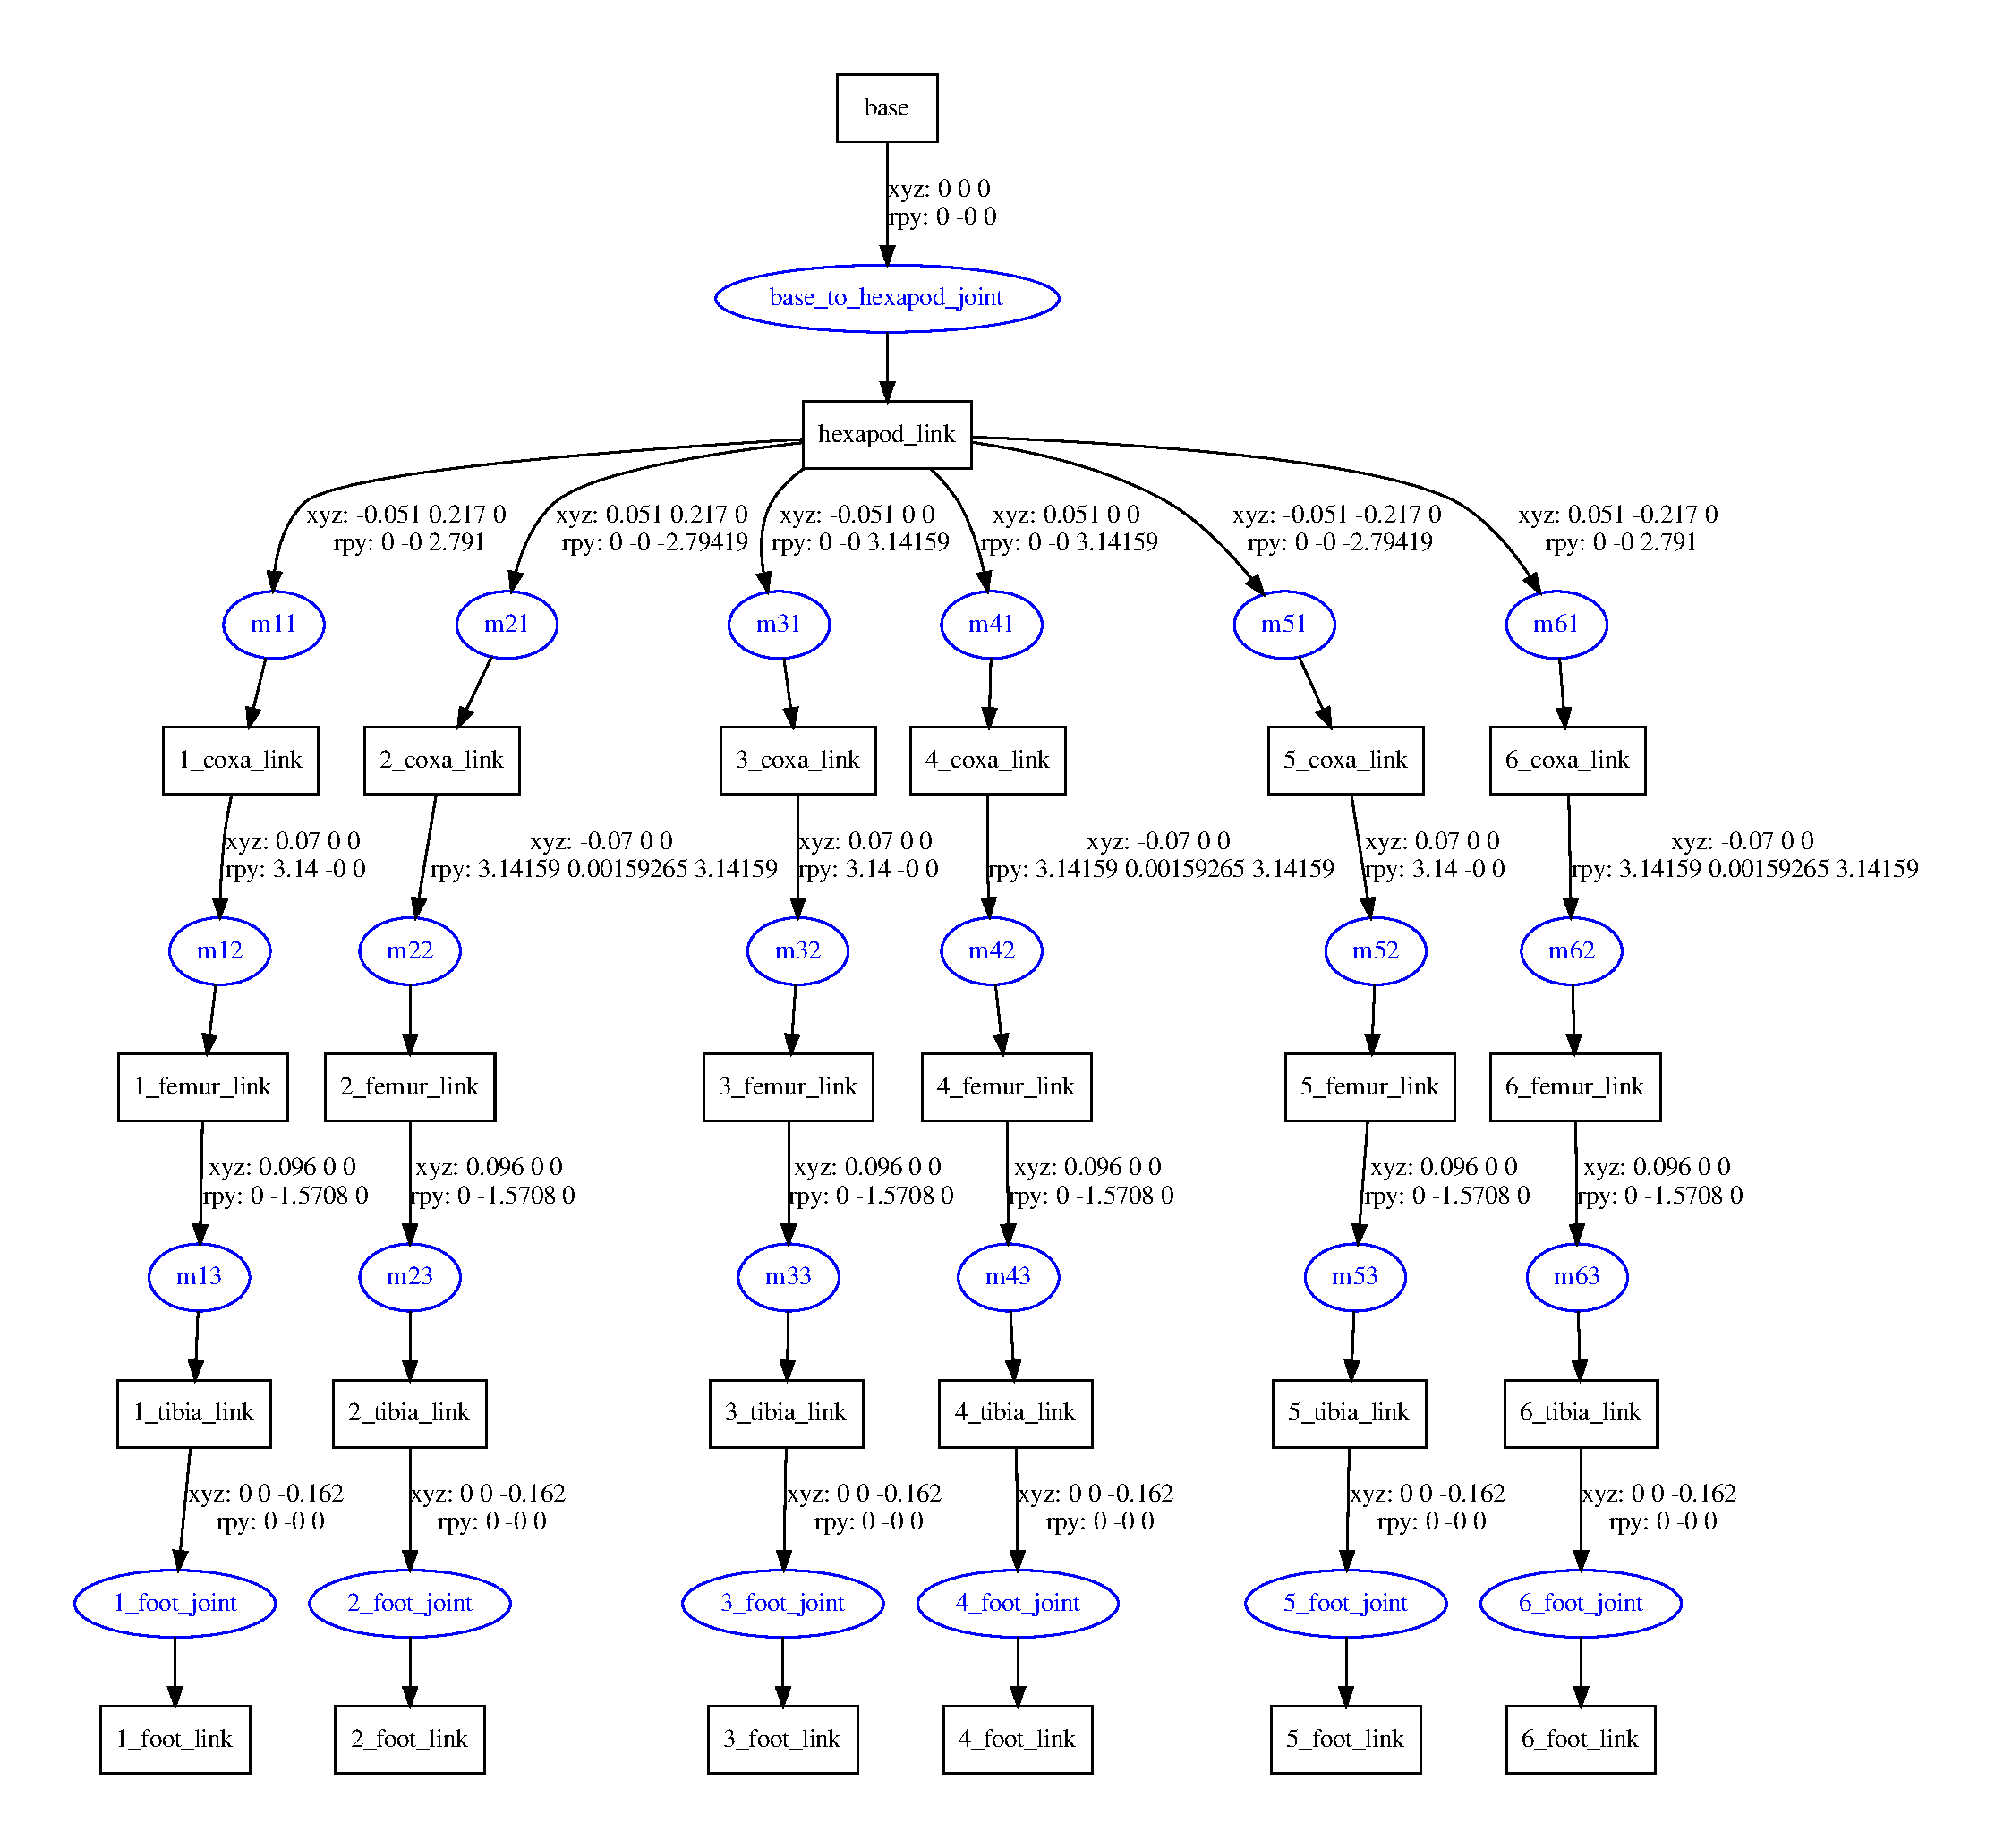
\includegraphics[height=8cm]{kapitel2/urdtographizakrobat}
  \caption{Darstellung des Transformationsbaums des Akrobats}
  \label{Kap2:urdtographizakrobat}
\end{figure}

\subsubsection{Robotermodell und tf-Framework}

Robotermodelle können in einem \ac{URDF} angegeben werden. Dieses Format beinhaltet jedes Segment und jedes Gelenk sowie deren Zusammenspiel. Dabei wird für jedes Segment die Visualisierung, die Massenträgheit sowie ein Kollissionsmodell angegeben. Die Visualisierung und die Kollission erfolgt beispielsweise über das Format \ac{STL}, aber auch, falls möglich, über einfache geometrische Objekte. Die Gelenke beinhalten den Verweis auf das Eltern- und auf das Kindelement sowie einen Arbeitsbereich. Eine Möglichkeit das \ac{URDF}-Format zu verbessern bieten \ac{Xacro}. \ac{Xacro} zielt vor allem darauf ab das Format lesbarer und kürzer zu gestalten. Über Tools wie den rviz, können Robotermodelle visualisiert werden. Mittels des Kommandozeilen-Tools urdf\_to\_graphiz lässt sich der Transformationsbaum eines Robotermodell visualisieren. Dies wird in \autoref{Kap2:urdtographizakrobat} am Beispiel des Akrobat dargestellt.

\subsection{Gazebo}

Die Entwicklung des Frameworks Gazebo von Dr. Andrew Howard und seinem Studenten Nate Koenig beginnt im Jahr 2002 an der University of Southern California. Seit dem wird das Projekt ständig weiterentwickelt. Gazebo ist eine Robotersimulation mit einer Physik-Engine und hoher Kompatibilität zu \ac{ROS}. Der folgende Abschnitt soll basiernd auf \autoref{Kap2:gazeboarchitektur} einen Überblick über die Architektur des Frameworks geben, das für den Laufplaner eingesetzt wird. \autocite{gazebosim} \autocite{Koenig-2004-394}

\begin{figure}[b!]
  \centering
  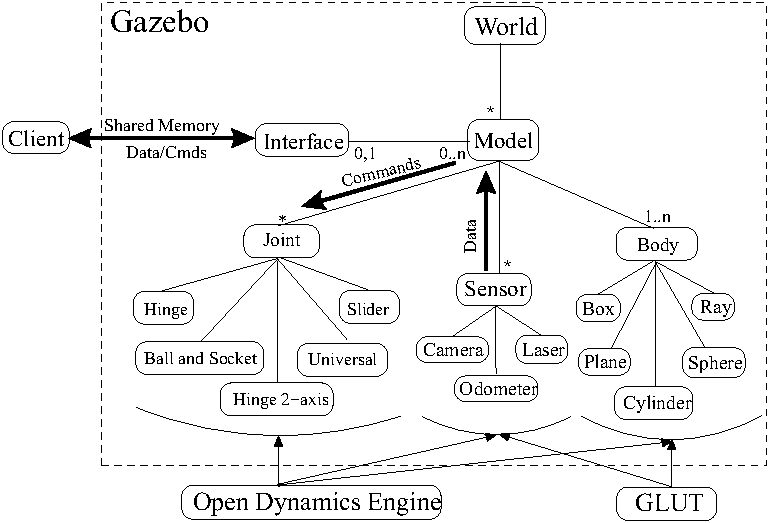
\includegraphics[height=10cm]{kapitel2/gazebo}
  \caption{Architektur des Gazebo-Frameworks \autocite{Koenig-2004-394}}
  \label{Kap2:gazeboarchitektur}
\end{figure}

\subsubsection{Physik-Engine}

Als Physik-Engine wird standardmäßig die \ac{ODE} genutzt. Es sind auch weitere Physik-Engines möglich, da diese nicht fest in der Architektur verdrahtet ist. Alternativ zum Standard können demnach Bullet, Simbody oder DART genutzt werden.
    
\subsubsection{Visualisierung}

Für die reine Visualisierung nutzt Gazebo standardmäßig OpenGL sowie GLUT (OpenGL Utility Toolkit). OpenGL ist plattformunabhängig, hochskalierbar, stabil und wird stetig weiterentwickelt. Außerdem sind viele Funktionalitäten in OpenGL auf Hardware-Ebene in der Grafikkarte entwickelt, so dass die CPU entlastet ist und andere Aufgaben schneller leisten kann.}

\subsubsection{Welt}

Die Gazebo-Welt ist eine Sammlung aus verschiedenen Komponenten:
\begin{itemize}
  \item \emph{Modelle}: Modelle sind Objekte mit einer physikalischen Definition.
  \item \emph{Körper}: Körper sind die grundlegenden geometrischen Bauteile beispielsweise des Roboters.
  \item \emph{Gelenke}: Gelenke verbinden die Körper miteinander und formen damit die möglichen kinematischen Bewegungen.
  \item \emph{Sensoren}: Ein Sensor in Gazebo ist ein abstraktes Gerät ohne physikalische Definition. Gazebo bietet aktuell einen Odometriesensor, einen Nähesensor sowie eine Kamera an.
\end{itemize}
  
\subsubsection{Erstellung von Modellen}

Aktuell müssen Modelle per Hand erstellt werden. Dies erfolgt in der Regel über das sdf-Format. Kommt \ac{ROS} zum Einsatz, kann mittels der Node urdf\_spawner auch das urdf-Format verwendet werden.}
  
Abschließend ist noch wichtig, dass Gazebo durch Plugins erweiterbar ist und eine umfangreiche Schnittstelle bietet, die in einem \ac{ROS}-Node mit C++ oder Python aufgerufen werden kann. Des Weiteren lässt Gazebo auch ein Rendering der Simulation auf einem Remote-Server zu, so dass verteilte Anwendungen möglich werden. Dies ist in vielen Fällen aufgrund begrenzter Rechenleistung von Vorteil. 